\documentclass[a4paper]{article}

% Global layout
\usepackage{fancyhdr, graphicx, hyperref, indentfirst, lastpage, setspace}
\usepackage{geometry}

% Encoding
\usepackage[utf8]{vntex, inputenc}
\usepackage[english]{babel}
\usepackage{amsmath, amssymb, gensymb}

% Better table
\usepackage{array, booktabs, multicol, multirow, siunitx, tabularx}

% Graphics
\usepackage{caption, float}

% Bullets & numbering
\usepackage{enumitem}

% Page setup
\allowdisplaybreaks{} % to have page breaks inside align* environment
\hypersetup{urlcolor=blue,linkcolor=black,citecolor=red,colorlinks=true}
% \usemintedstyle{emacs}
\numberwithin{equation}{section}
\renewcommand{\arraystretch}{1.2} % space between table rows

% Global style setup
\makeatletter % change font size for not having underfull hbox
\renewcommand\Huge{\@setfontsize\Huge{22pt}{18}}
\makeatother

\AtBeginDocument{\renewcommand*\contentsname{Contents}}
\AtBeginDocument{\renewcommand*\refname{References}}
\setlength{\headheight}{40pt}
\pagestyle{fancy}
\fancyhead{} % clear all header fields
\fancyhead[L]{
  \begin{tabular}{rl}
    \begin{picture}(25,15)(0,0)
    \put(0,-8){
\includegraphics[width=8mm, height=8mm]{./assets/hcmut.png}}
    \end{picture}
    \begin{tabular}{l}
      \textbf{\bf \ttfamily University of Technology, Ho Chi Minh City}\\
      \textbf{\bf \ttfamily Faculty of Computer Science and Engineering}
    \end{tabular}
  \end{tabular}
}
\fancyhead[R]{
	\begin{tabular}{l}
		\tiny \bf \\
		\tiny \bf
	\end{tabular}  }
\fancyfoot{} % clear all footer fields
\fancyfoot[L]{\scriptsize \ttfamily Programming Integration Project --- Academic year 2021--2022}
\fancyfoot[R]{\scriptsize \ttfamily Page {\thepage}/\pageref{LastPage}}
\renewcommand{\headrulewidth}{0.3pt}
\renewcommand{\footrulewidth}{0.3pt}

% \everymath{\color{blue}}

\newcommand*\mean[1]{\bar{#1}}

\begin{document}

\begin{titlepage}
  \begin{center}
    VIETNAM NATIONAL UNIVERSITY, HO CHI MINH CITY \\
    UNIVERSITY OF TECHNOLOGY \\
    FACULTY OF COMPUTER SCIENCE AND ENGINEERING
  \end{center}

  \vspace{1cm}

  \begin{figure}[H]
    \centering
    
\includegraphics[width=0.4\textwidth]{./assets/hcmut.png}
  \end{figure}

  \vspace{1cm}

  \begin{center}
    \begin{tabular}{c}
      \textbf{\Large Programming Integration Project (CO3103)} \\
      {}                                                       \\
      \midrule                                                 \\
      \textbf{\Large Project Report}                           \\
      {}                                                       \\
      \textbf{\Huge Mobile Phone Selling Webapp}               \\
      {}                                                       \\
      \bottomrule
    \end{tabular}
  \end{center}

  \vspace{3cm}

  \begin{table}[h]
    \begin{tabular}{rll}
      \hspace{5cm} Advisor:  & Prof.\ Quản Thành Thơ &         \\
      \hspace{5cm} Students: & Nguyễn Hoàng          & 1952255 \\
                             & Nguyễn Chính Khôi     & 1952793 \\
                             & Vũ Anh Nhi            & 1952380 \\
                             & Lương Duy Hưng        & 1952747 \\
    \end{tabular}
  \end{table}

  \begin{center}
    {\footnotesize HO CHI MINH CITY, DECEMBER 2021}
  \end{center}
\end{titlepage}

\tableofcontents
\newpage

\section{Topic}
This project focuses on creating a web-based application that allows users or customers to browse and make transactions.
The specific target of product is phone, primarily smart mobile devices.

This e-commerce application is analogous to real life phone selling retailers that require a more convenient and efficient way for customers to interact with their products.
Because of that, the requirements and features will mainly focus on practical demands as if it was proposed to solve the problem.

\subsection{Proposed workload}
\begin{center}
  \begin{tabular}{*{3}{l}}
    \toprule
    Task                    & Component           & Member        \\
    \midrule
    Database                & Backend             & Hoàng         \\
    Deployment              & Backend \& Frontend & Hoàng         \\
    Create mock-up homepage & Frontend            & Nhi           \\
    Codebase implementation & Backend             & Hưng \& Hoàng \\
    Codebase implementation & Frontend            & Khôi \& Nhi   \\
    \bottomrule
  \end{tabular}
\end{center}

\subsection{Proposed Features}
\begin{itemize}
  \item Authentication: Sign in and sign up, SSO optional
  \item Homepage: Display list of products
  \item Cart: Store items
\end{itemize}

\subsection{Feature details}
\begin{itemize}
  \item Menubar: Half left shows sections like products, brands, etc.; right portion has user's avatar and button for cart
  \item Authentication: On mouse hover over the user's avatar shows a drop-down list; if the user is signed in, this list will show a button to sign out, else show sign in and sign up buttons
  \item Authentication pages: Sign in and sign up have dedicated pages, with placeholder for SSO in the case we can implement it
  \item Homepage: Show some news divided by brands or the site's news
  \item Products page: Show about 20 products; allow usage for filter and sort
  \item Item page: Show all information about the item like colors, memory options, etc.; add placeholder for other recommended items
  \item Cart button: With small number indicating total number of items in cart; on mouse hover shows a truncated drop-down list of cart
  \item Cart page: Shows all item in cart; allows changing properties like colors, quantity, etc.; calculate total price by item choice and overall
\end{itemize}

\newpage

\section{Technologies \& Features}
So far, we have been learning about the thinking process of a developer.
For this integration project, we decided to practice this thinking process using some new frameworks.
At this point, we have already picked our tools, and after hours of research, we draw the conclusion on how all these technologies work and work together.

\subsection{Frontend: Reactjs}

\includegraphics[width=\textwidth]{assets/reactjs-logo.png}

React (React.js or ReactJS) is a free and open-source front-end JavaScript library for building user interfaces or UI components.
Developed at Facebook and released in 2013, it can be said that React has been the most influential UI library of recent years.

We use React to build components that represent logical reusable parts of the UI\@.
The beauty of React is that the simplicity of building a component has been brought down to its theoretical minimum: a Javascript function.
The return value from these functions is the HTML or UI, which is written in a special syntax called JSX, allowing easy combination of Javascript with Html markup.

The main reason we want to use React is not the library itself but the massive ecosystem surrounding it.
React itself does not care about routing state management, animation or anything like that.
Instead, it lets those concerns evolve naturally within the open-source community.
No matter what we are trying to do, there is a good chance that a good supporting library to help us get it done has already existed.

\subsubsection{Component Reuse}
Why would you constantly reinvent the wheel when you can simply reuse code that has already been written and tested by other developers?

ReactJS introduces the so-called components, which make it possible to split the UI into independent, reusable pieces, and think about each piece in isolation.

For instance, we can have a button component display with different colors in several parts of our application.
Although it is the same button component when we provide it with a data set (e.g color, or a function), it modifies itself and outputs a UI instance of the element.

This pattern of creating React components is necessary for scaling.
It helps save time by ensuring less code is written, development is faster, the code base is simpler, and maintenance is stress-free.

\subsubsection{Virtual DOM}
The Document Object Model (DOM) is an application programming interface that represents an XML document as a tree structure wherein each node is an object representing a part of the document.

Most often it's inefficient and slow because it's necessary to recalculate the CSS, recreate the layout, and essentially repaint the entire web page every time the DOM changes.

ReactJS overcomes the DOM's inefficiencies by using the so-called Virtual DOM\@.

Just like the actual DOM, the Virtual DOM represents all elements and their attributes as a node tree.
When something changes, React JS updates the Virtual DOM and figures out how it differs from the actual DOM, updating the actual DOM only with what has actually changed.

\subsubsection{JSX}
ReactJS introduces another concept called JSX, and it is a syntax extension to JavaScript.

React embraces the fact that rendering logic is inherently coupled with other UI logic: how events are handled, how the state changes over time, and how the data is prepared for display.

Instead of artificially separating technologies by putting markup and logic in separate files, React separates concerns with loosely coupled units called “components” that contain both.

React doesn't require using JSX, but most people find it helpful as a visual aid when working with UI inside the JavaScript code.
It also allows React to show more useful error and warning messages.

\subsection{Backend: Django}

\includegraphics[width=\textwidth]{assets/dj-logo.png}

Django is a high-level Python web framework that encourages rapid development and clean, pragmatic design.
Built by experienced developers, it takes care of much of the hassle of web development, so you can focus on writing your app without needing to reinvent the wheel.

\subsubsection{Django REST framework}
Django REST framework is an open-source application platform that allows developers to build applications on top of the REST framework without having to worry about the infrastructure being compromised.
Django REST framework supports multiple languages including JavaScript which we use for Reactjs and provide complete solution for managing data using Serializers.

\subsubsection{Architecture}
For the sake of this project, we decided to build this website using the simplest architecture: the \texttt{MVC}.

\texttt{MVC} stands for Model-View-Controller and have the most basic interactions between \texttt{Model} at the backend and \texttt{View} at the frontend through a medium \texttt{Controller}.
Technically, the request of the user is captured by the Controller, it then calls the database to retrieve the the corresponding object(s) and return it in form of JSON/XML\@.

For example, when a user presses a button ``Apple'' in the Homepage \texttt{View}, a corresponding action in \texttt{Controller} will be triggered and retrieve all the mobile phones whose manufacturer is ``Apple'' using the predefined \texttt{Model}.
Otherwise, the HTTP mechanism will return an error page.

\subsubsection{Serializers}
Serialization is a common terminology that is not new to Web Programming.
To implements serialization, we use a so-called \texttt{Serializer}.

Serializers in Django REST Framework are responsible for transforming objects into data types that are understandable in JavaScript and the front-end framework.
The serializer also provides deserialization, allowing the parsed data to be reverted to a complex type after the received data is first validated.

In our website, we prefer \texttt{ModelSerializer} rather than regular \texttt{Serializer} as it has some of the following advantages:
\begin{enumerate}
  \item It auto-generates a set of fields that is specified by the Model we created.
  \item It provides some validators for serialization such as unique\_together.
  \item It contains some of the default function like create(), save() for the ease of storing data.
\end{enumerate}

\subsection{Database}

\includegraphics[width=\textwidth]{assets/postgresql-logo.png}

PostgreSQL is a powerful, open source object-relational database system that uses and extends the SQL language combined with many features that safely store and scale the most complicated data workloads.

With more than 30 years of active development on the core platform, PostgreSQL has earned a strong reputation for its proven architecture, reliability, data integrity and more.

\newpage

\section{UI and screen flow}

\subsection{Mock-up}

We have sketched the design of four pages that is in the scope of this project.
They are the \texttt{Home} page, \texttt{Product List} (displaying list of products) page, \texttt{Product Detail} page, and \texttt{View Cart} page.
We also sketched the \texttt{log-in} pop-up window if customers clicked on the icon, and the \texttt{show-cart} pop-up window if you hover the mouse to the cart icon on the navigation bar.\\

\begin{figure}[H]
  \centering
  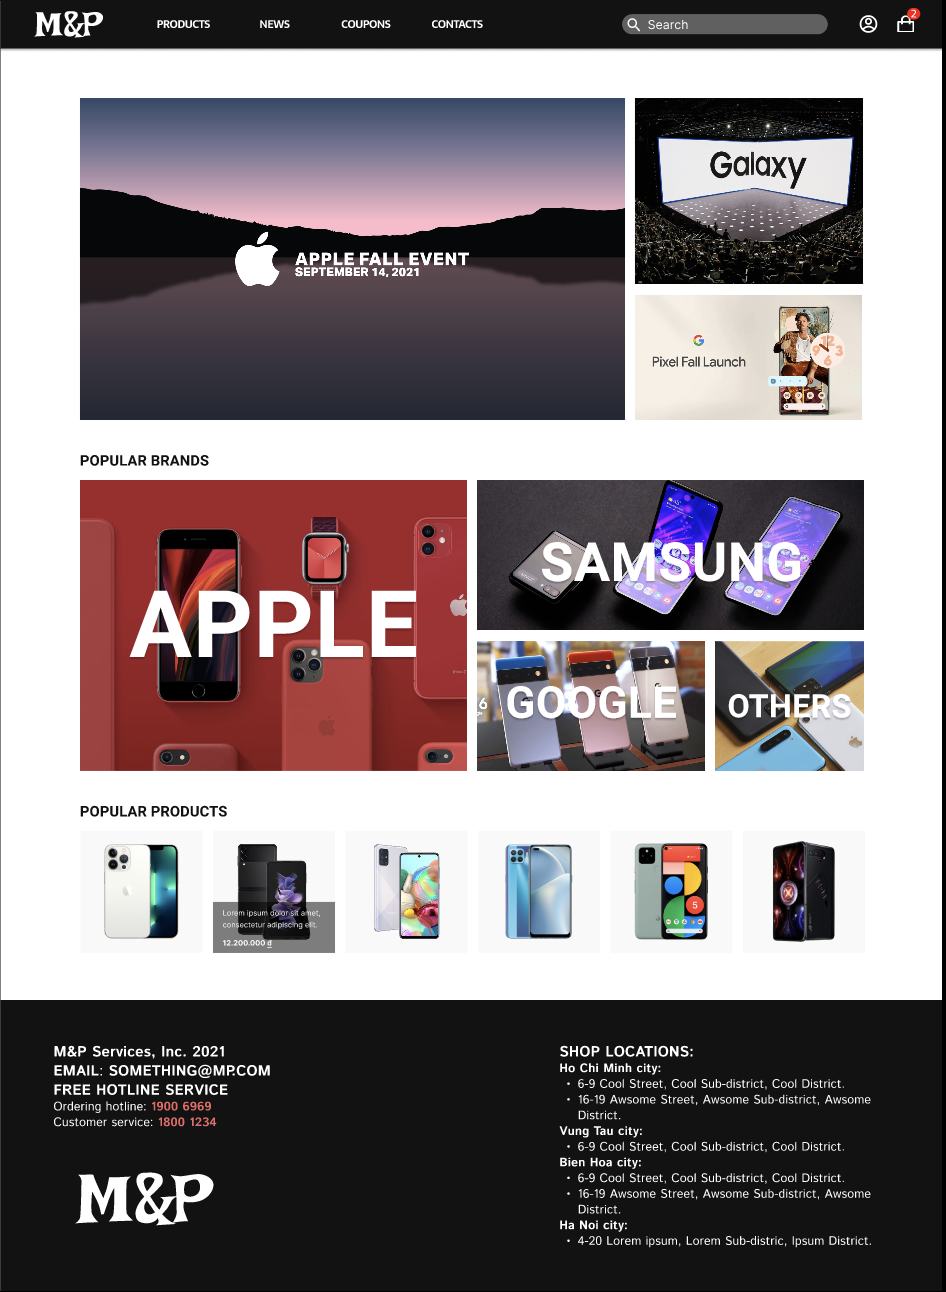
\includegraphics[width=0.65\textwidth]{assets/p2/p1.png}
  \caption{Home Page}
\end{figure}

These are the screenshots of the pages we designed using \texttt{Figma}.
\texttt{Figma} is a vector graphics editor and prototyping tool, which is suitable for basic UI design.
For a higher resolution view, please see the link \href{https://www.figma.com/proto/VaFUVfikhd1N98XmaqhA4p/Mock-up?node-id=35\%3A2504&scaling=scale-down-width&page-id=0\%3A1}{Mock-up}.

\begin{figure}
  \centering
  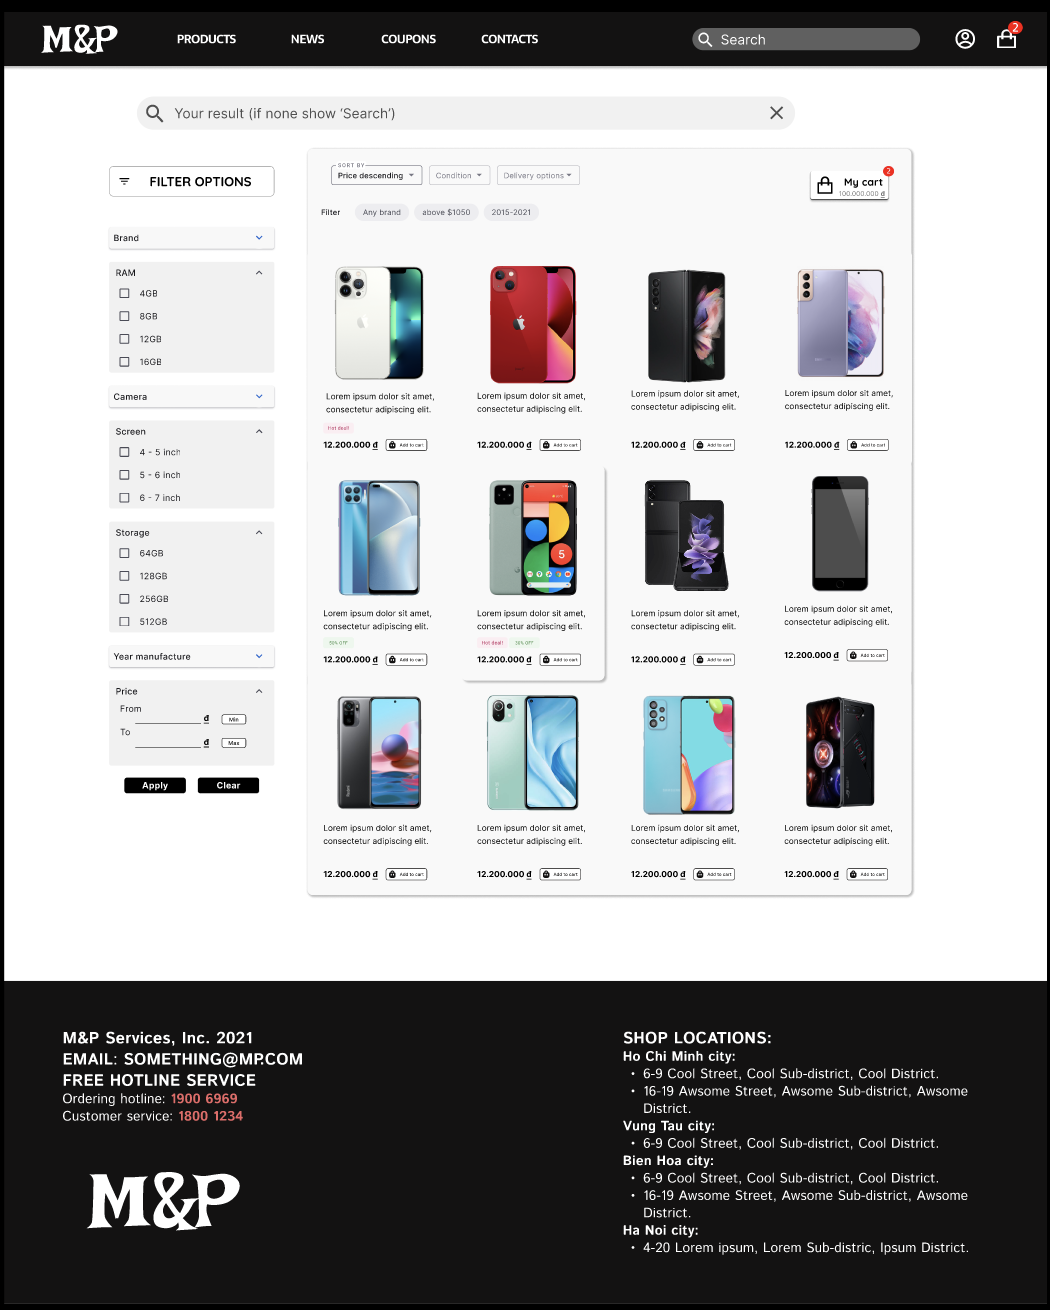
\includegraphics[width=0.9\textwidth]{assets/p2/p2.png}
  \caption{Product List Page}
\end{figure}

\begin{figure}
  \centering
  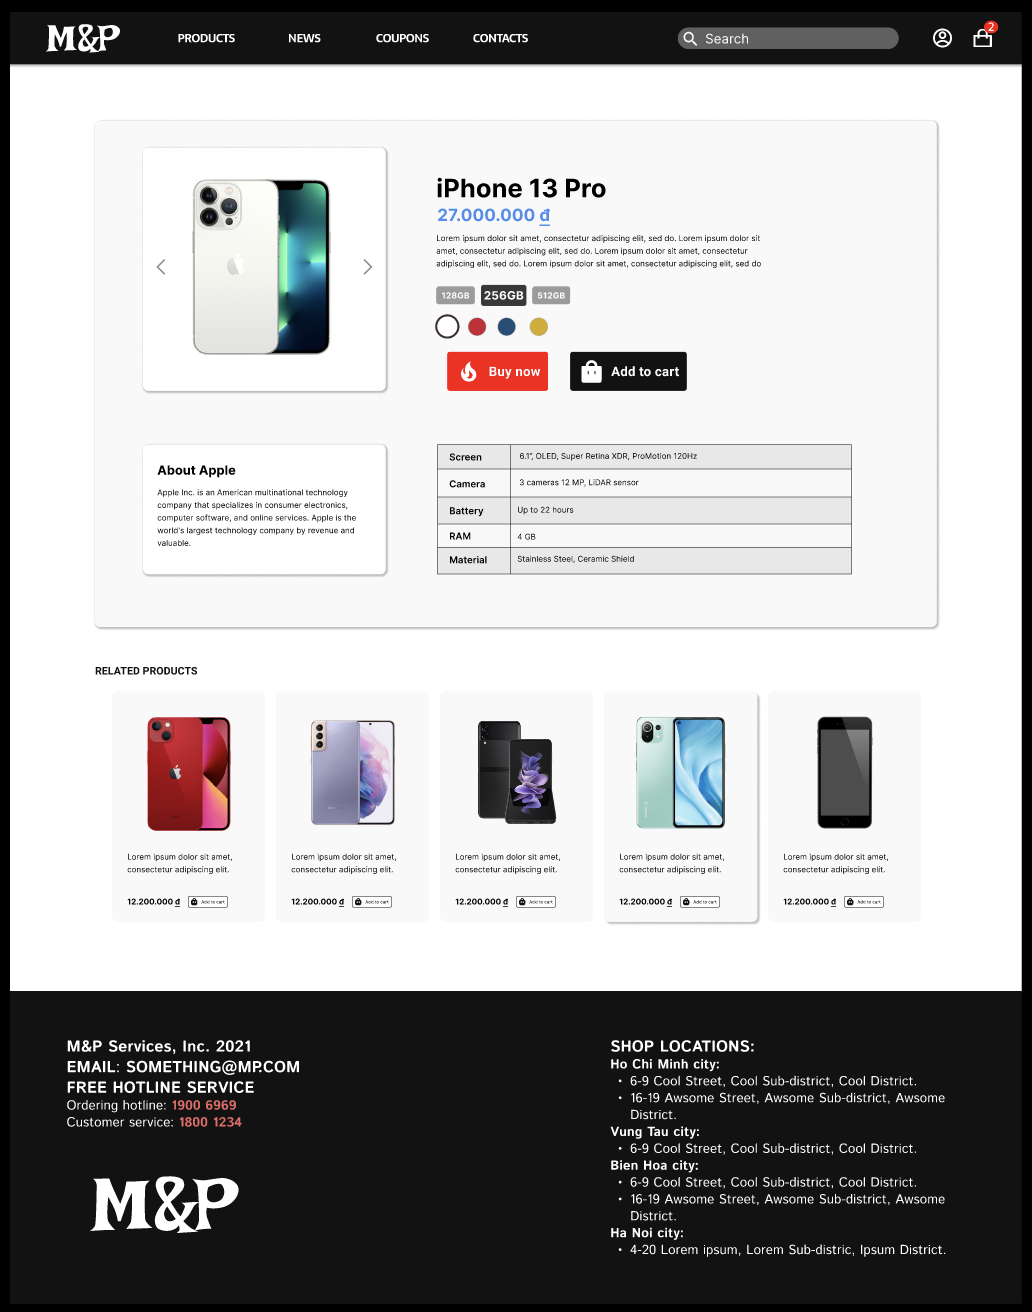
\includegraphics[width=0.9\textwidth]{assets/p2/p3.png}
  \caption{Product Detail Page}
\end{figure}

\begin{figure}
  \centering
  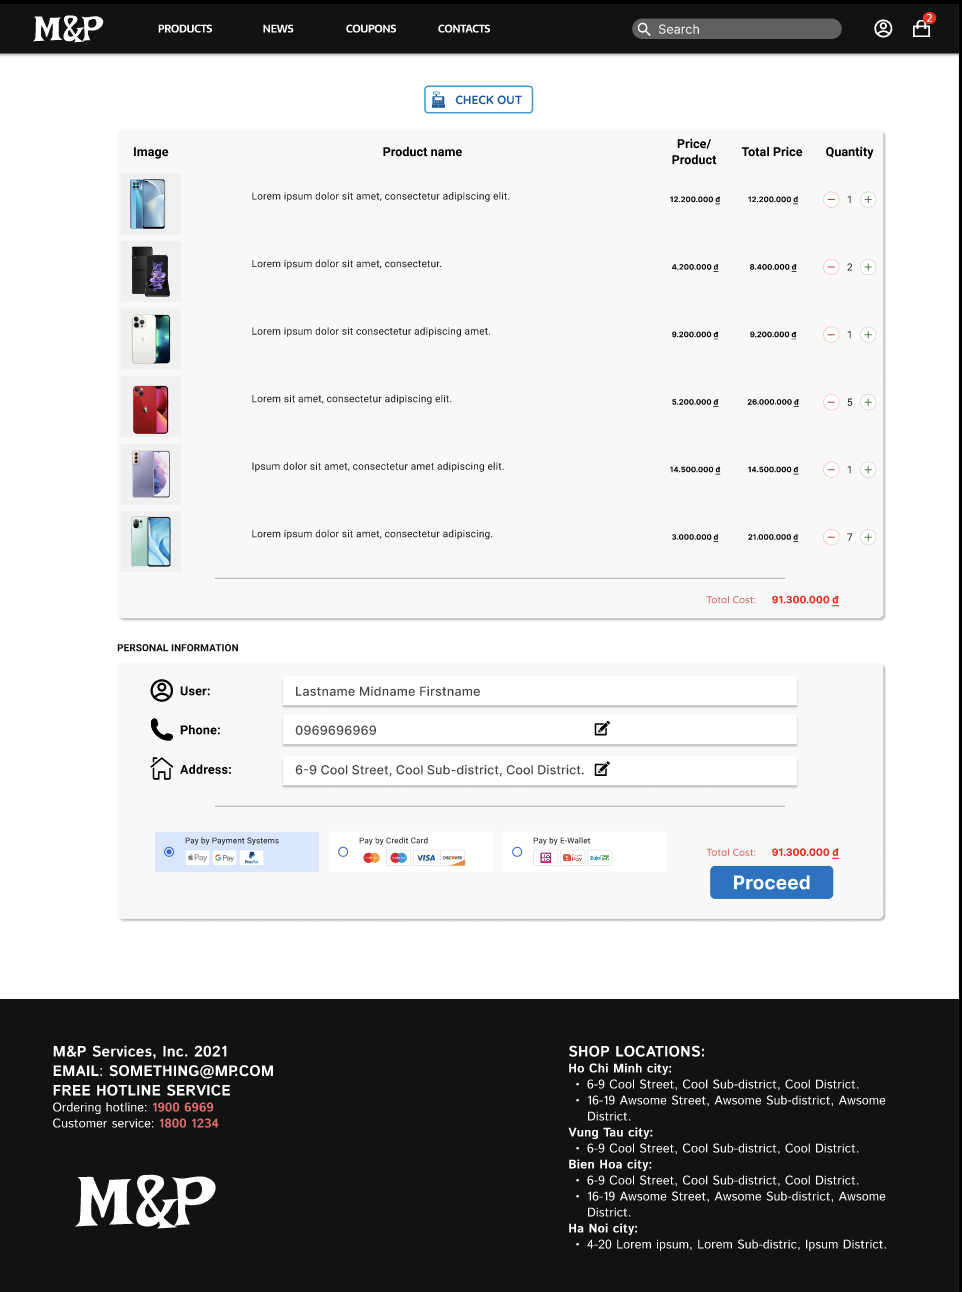
\includegraphics[width=0.9\textwidth]{assets/p2/p4.png}
  \caption{Check Out Page}
\end{figure}

\newpage
\subsection{Screen Flow}

This is the general screen flow of the website.
Most of the pages are linked by the buttons on the navigation bar.

\begin{figure}[H]
  \centering
  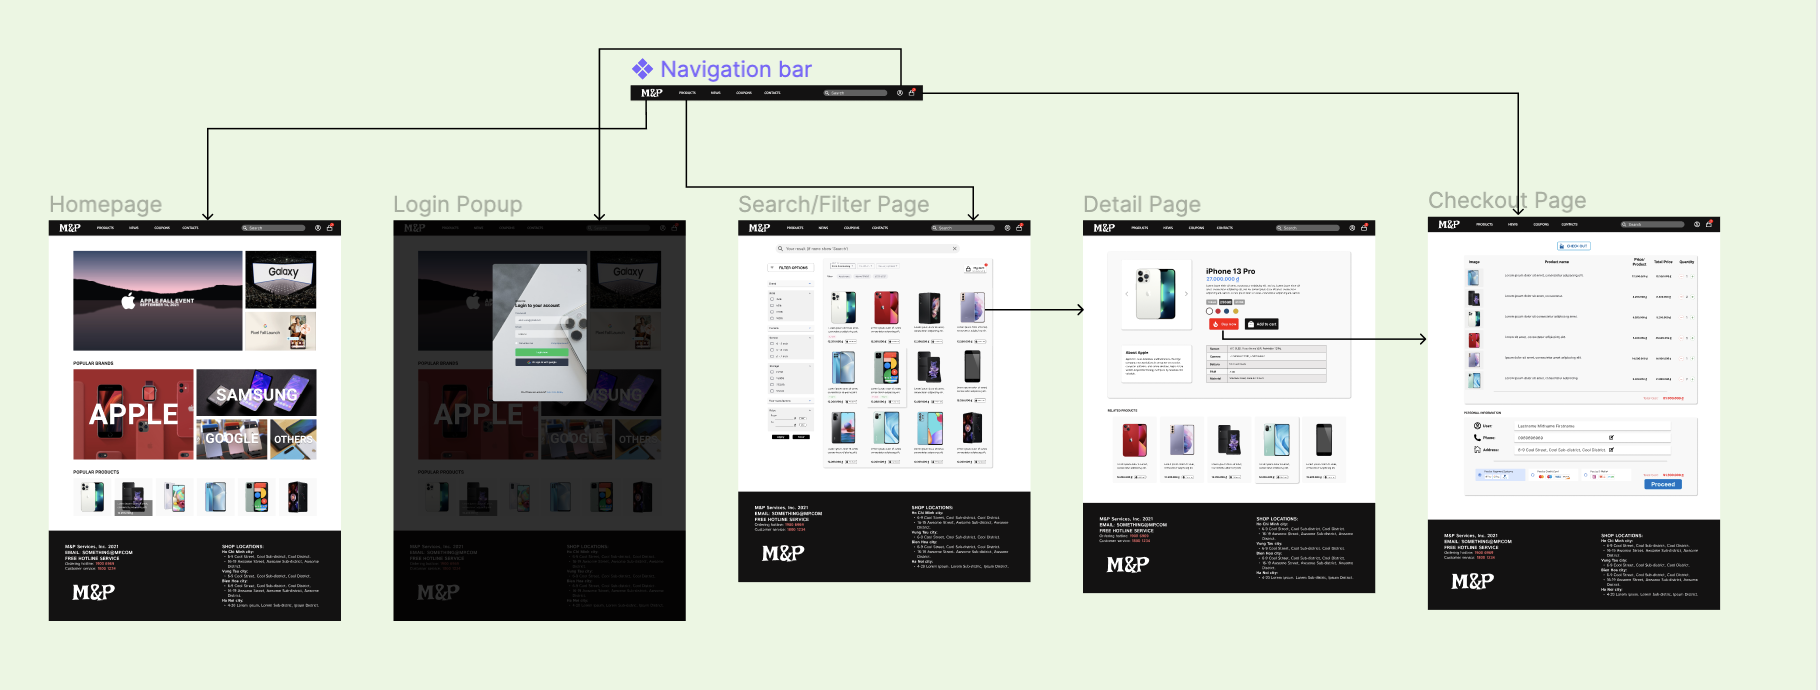
\includegraphics[width=1\textwidth]{assets/p2/screenflow.png}
  \caption{General screen flow}
\end{figure}

We also drew a flow chart to represent the normal flow when a customer navigates through the website.
The boxes in green are the pages associated with a destination, and the blue ones are the pop-ups that can appear on top of any page when we click the icon in the navigation bar.
Both are components of the website.
The yellow diamonds show some decisions that need to be made.

\begin{figure}[H]
  \centering
  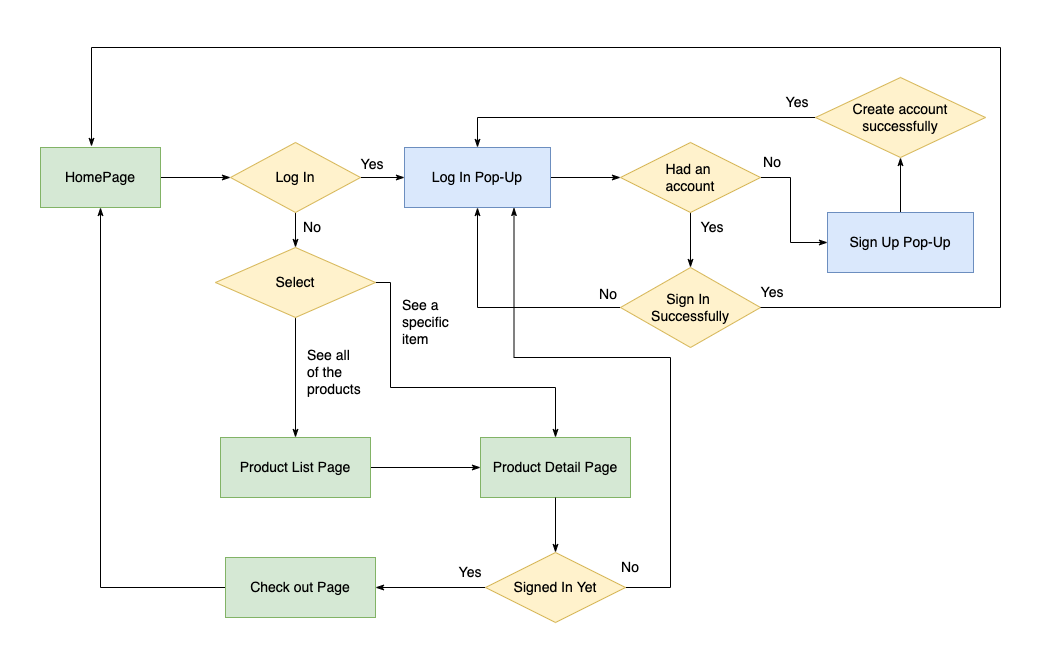
\includegraphics[width=0.9\textwidth]{assets/flow/flow-chart.png}
  \caption{The normal flow}
\end{figure}

The normal flow does not contain all possibilities when navigating.
This is mostly because the customers can opt out of the flow and choose the page that they want to visit by clicking the options on the navigation bar or enter the correct {\tt URL}.
This gives the customers much more freedom when visiting the website.

This also does not interrupt the main flow of the website.
Two important states (whether the customer is signed in or not, and what items do they have in their cart) are managed.
Therefore, it is not necessary to be worried if the customer choose not to go strictly the same as the normal flow.

\newpage

\section{Feature details}

\subsection{Home Page}

The {\tt Home Page} is similar to the UI design.
Some animations and features are also added.
If a user click on a brand, such as {\tt Apple}, he/she will be directed to a page that only shows the products of the respective brand.

\begin{figure}[H]
  \centering
  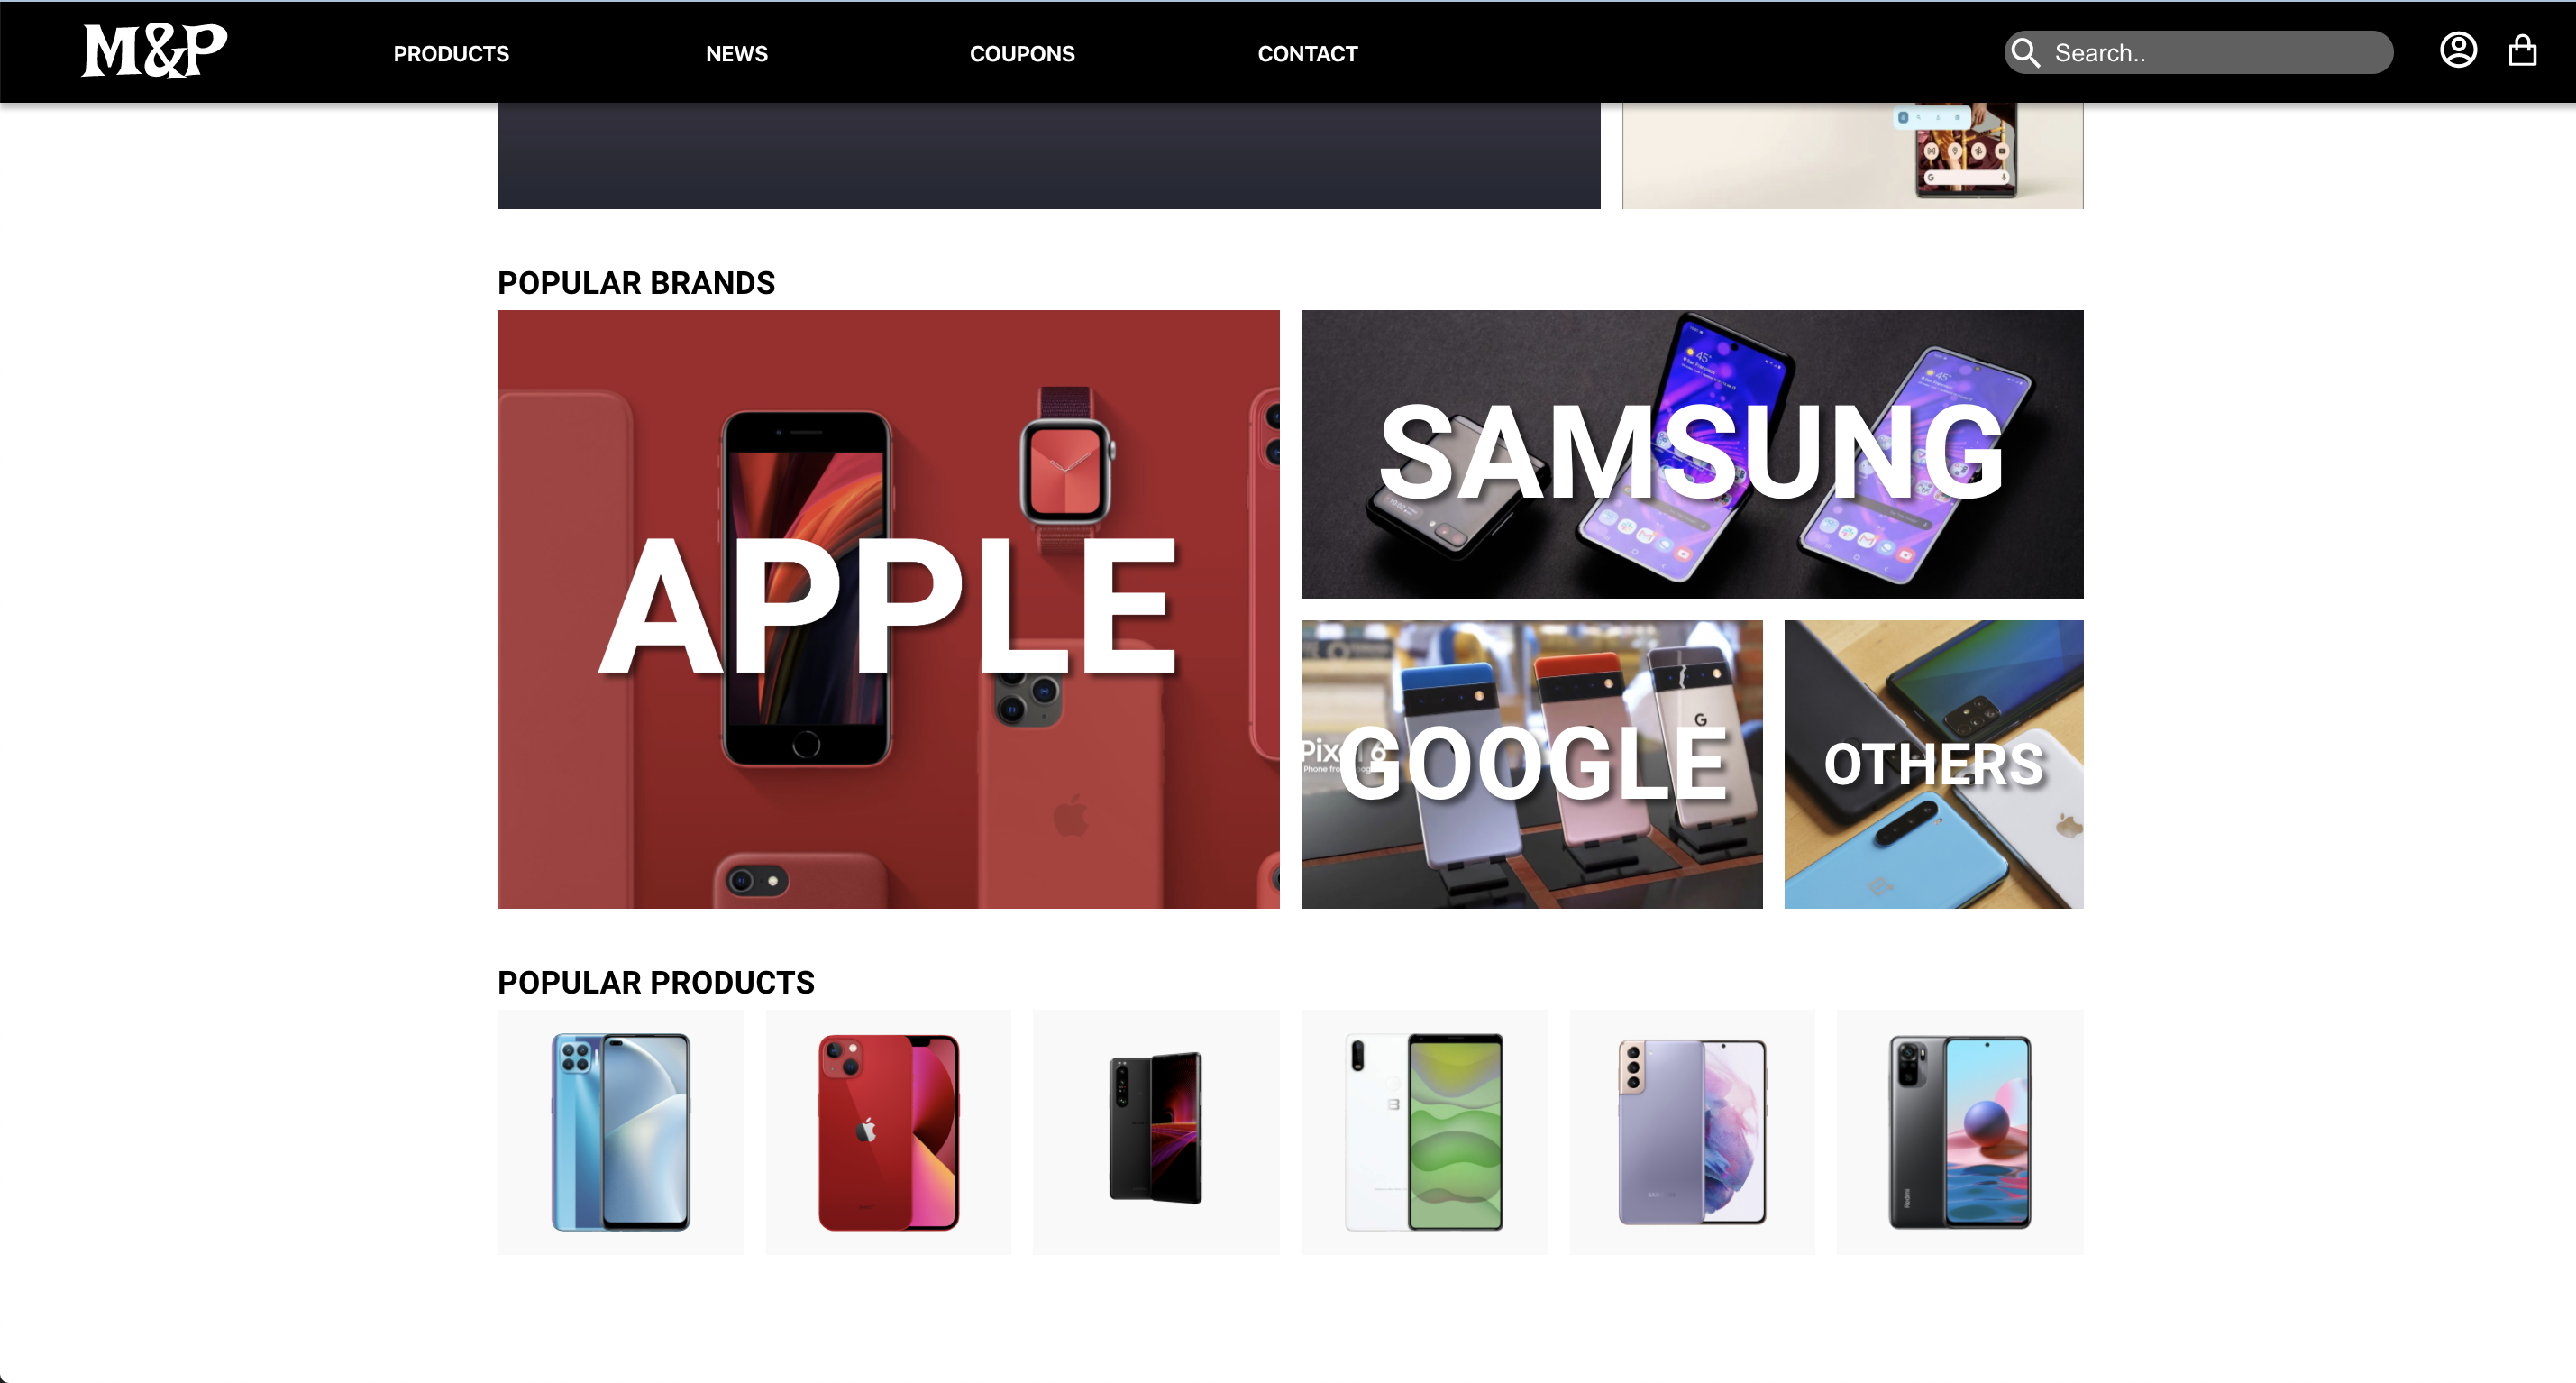
\includegraphics[width=0.9\textwidth]{assets/flow/home.png}
  \caption{Home Page}
\end{figure}

If a user hover on a product image, the name and price of the product will pop up.
If he/she click on the image, he/she will be directed to the detail page of the respective product.

\begin{figure}[H]
  \centering
  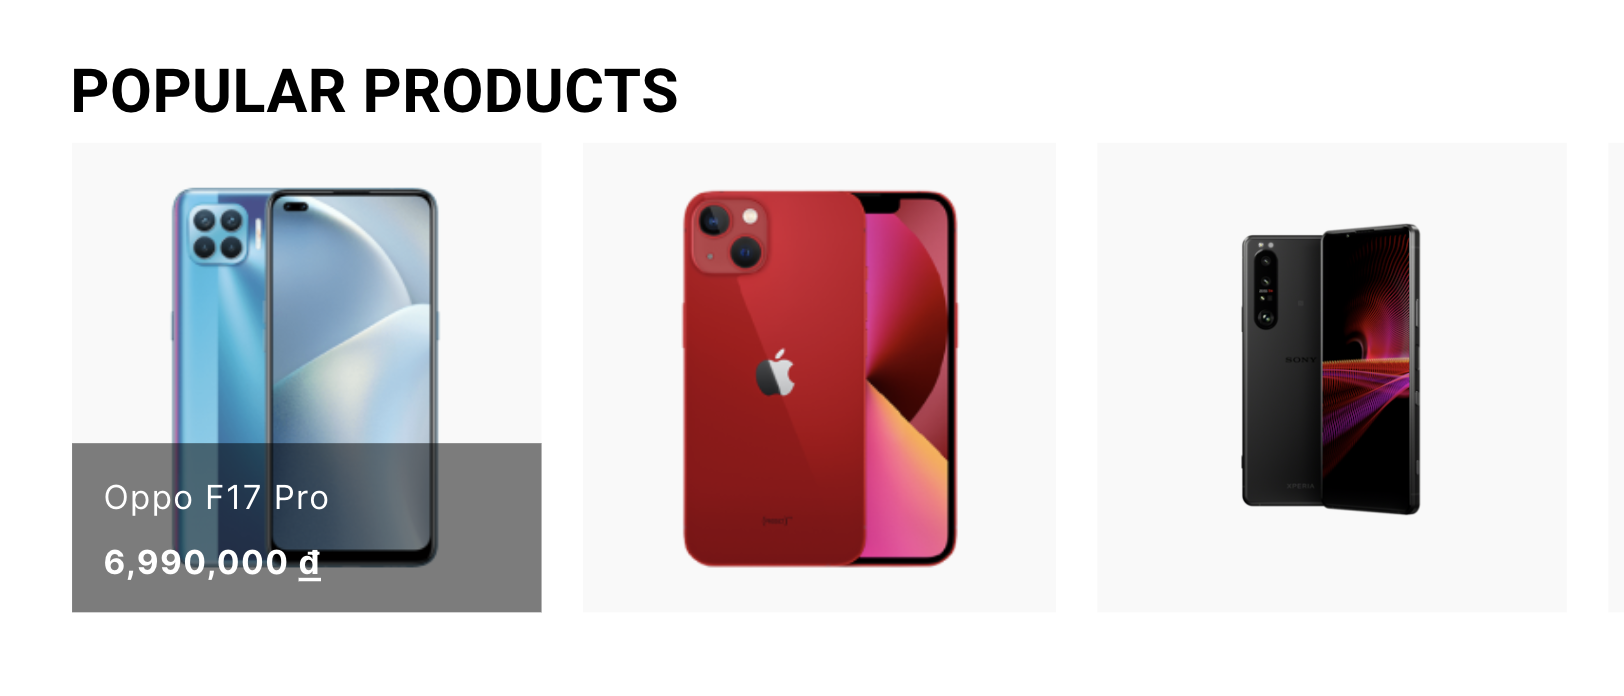
\includegraphics[width=0.9\textwidth]{assets/flow/product-pop.png}
  \caption{Popular Products}
\end{figure}

\subsection{Navigation bar}

The navigation bar contains the link to all of the essential pages.
We have implemented the destinations for the {\tt PRODUCTS} and {\tt M\&P} text.
The {\tt NEWS, COUPONS, CONTACT} text are just for presentation and are out of our project scope.

\begin{figure}[H]
  \centering
  
\includegraphics[width=0.9\textwidth]{assets/flow/navbar.png}
  \caption{Navigation bar}
\end{figure}

The {\tt search bar, account, view cart} icons are all usable.
When searching by typing in {\tt iphone}, the products showing are filtered to only phones that have the keyword in their names.
\begin{figure}[H]
  \centering
  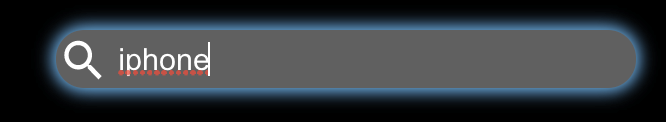
\includegraphics[width=0.5\textwidth]{assets/flow/search.png}
  \caption{Search bar}
\end{figure}

\begin{figure}[H]
  \centering
  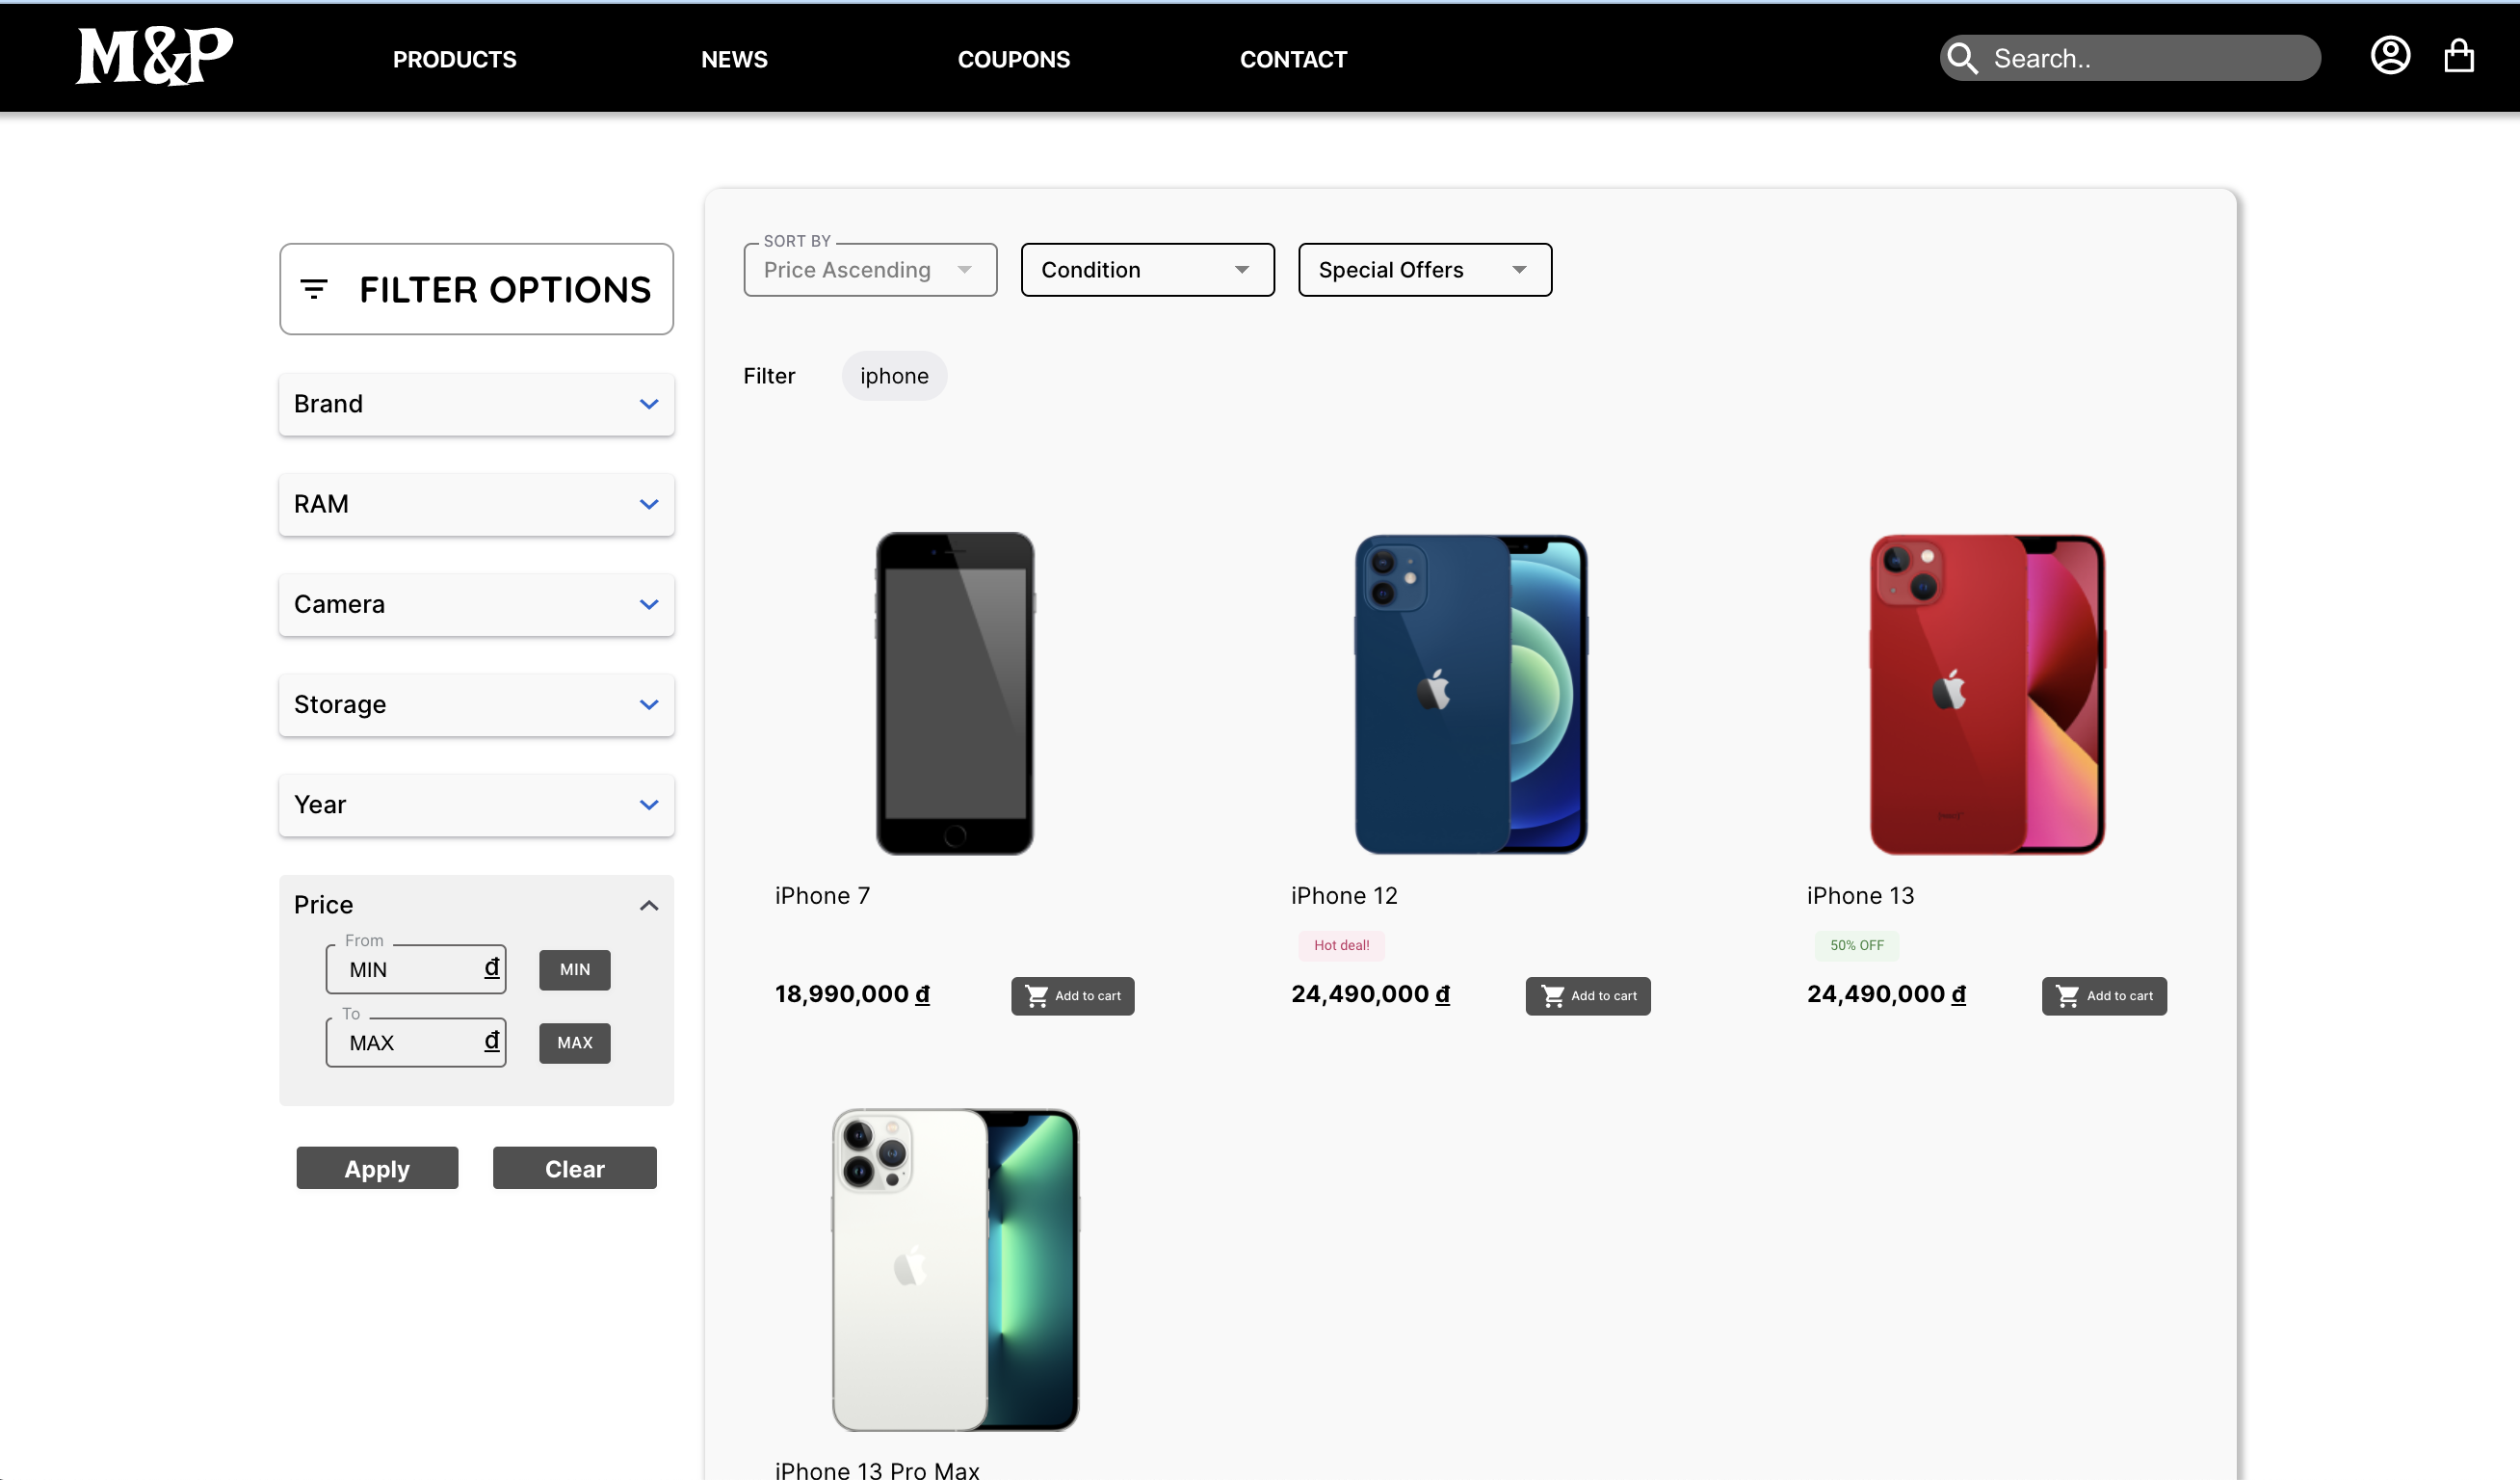
\includegraphics[width=0.9\textwidth]{assets/flow/iphone.png}
  \caption{List of the iPhones after searching}
\end{figure}

By clicking on the {\tt cart} icon, a summary of the cart shows up like this.
The cart contains one or more products only when users have successfully signed in and some items are added to the cart.

\begin{figure}[H]
  \centering
  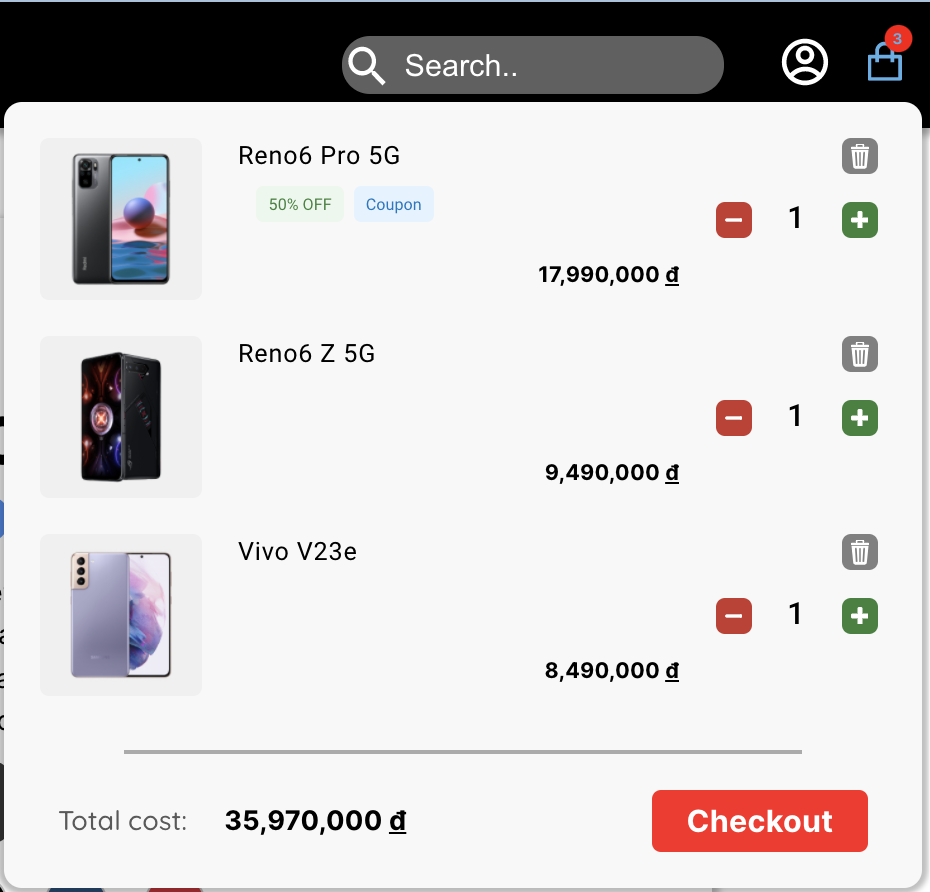
\includegraphics[width=0.5\textwidth]{assets/flow/cart-button.png}
  \caption{Cart summary}
\end{figure}

\subsection{Authentication}

If a user is not logged in, a list of {\tt Sign In} and {\tt Sign Up} options appeared.
By clicking in either option, a corresponded pop-up will show up.
If the user is logged in, there will only be one option {\tt Sign Out} displayed here.

\begin{figure}[H]
  \centering
  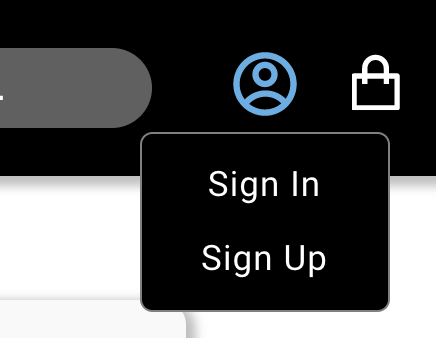
\includegraphics[width=0.5\textwidth]{assets/flow/not-signin.png}
  \caption{Sign In/ Sign Up Options}
\end{figure}

This is the sign-in form.
If a user have successfully created an account on the website, he/she can input the email and password to sign in to the page.
If not, he/she can click on the {\tt Join free today} link, and a sign-up form will appear.

\begin{figure}[H]
  \centering
  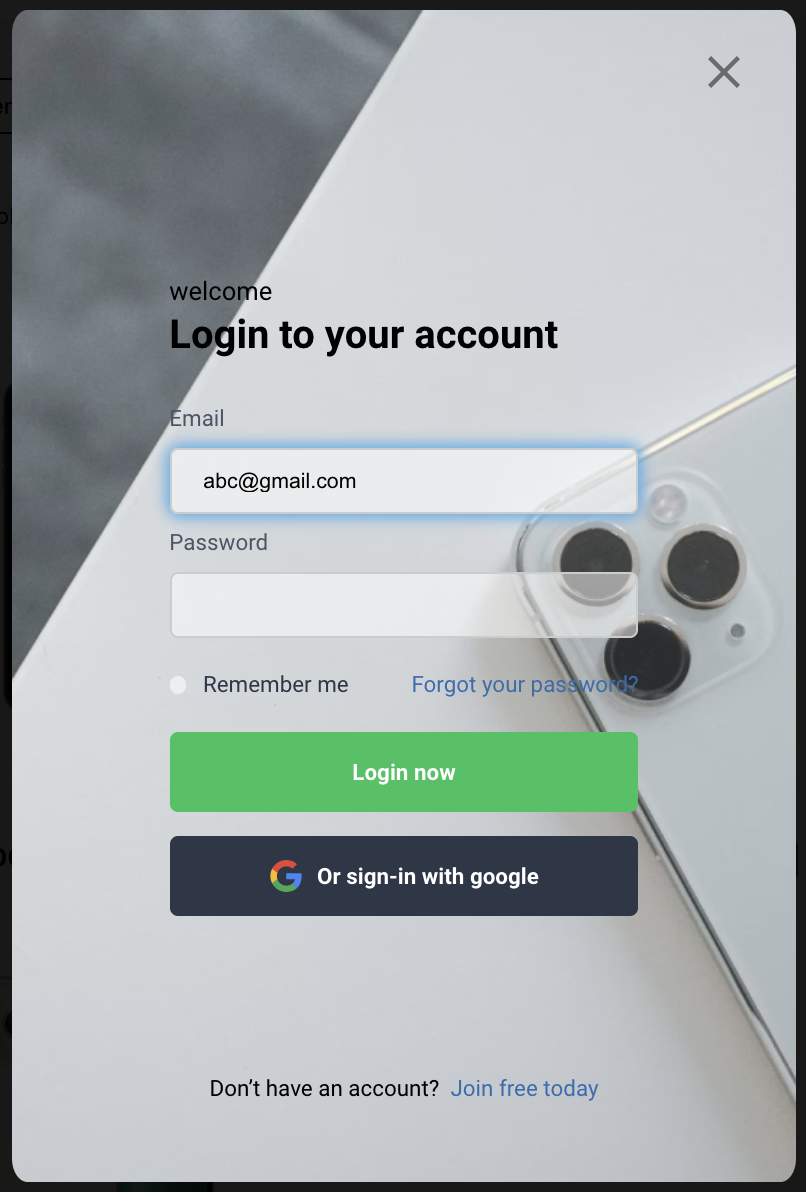
\includegraphics[width=0.4\textwidth]{assets/flow/signin.png}
  \caption{Sign In Form}
\end{figure}

\begin{figure}[H]
  \centering
  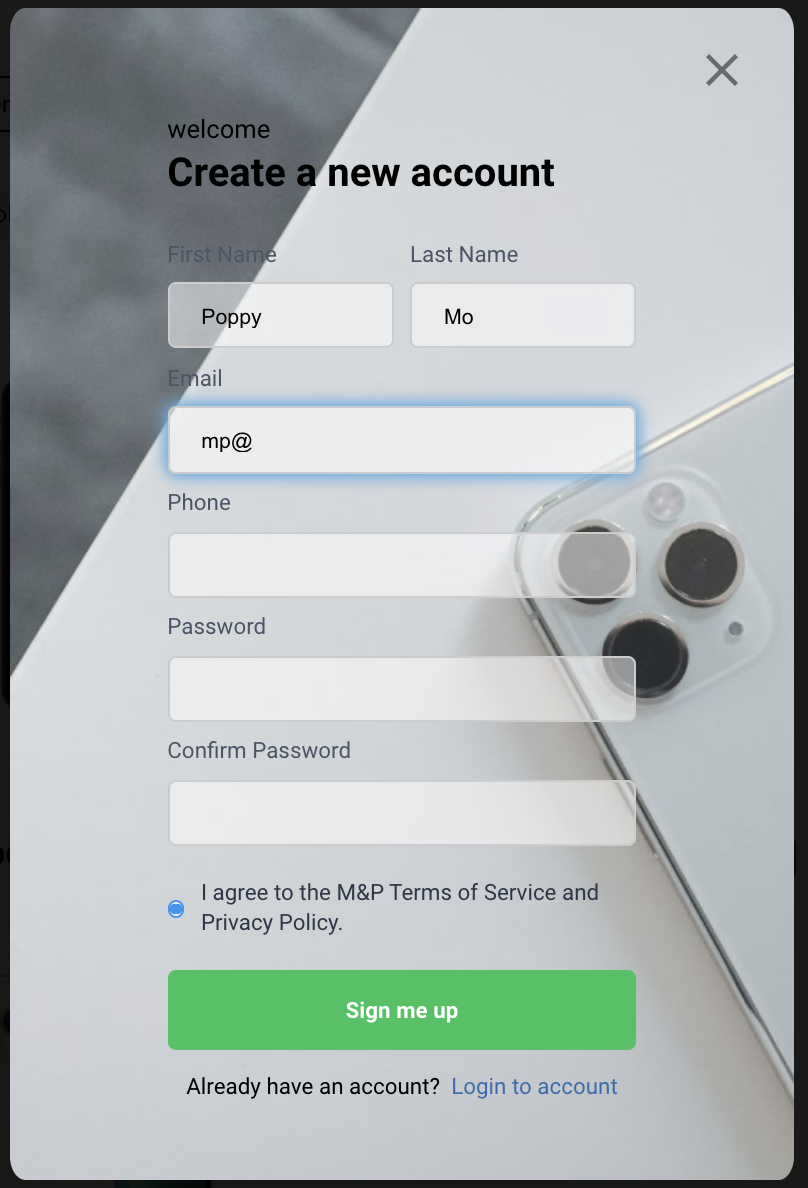
\includegraphics[width=0.4\textwidth]{assets/flow/signup.png}
  \caption{Sign Up Form}
\end{figure}

\newpage
\subsection{Product List Page}

This is the page that shows the list of the products.
Based on the filter options, it can show different sets of products.

\begin{figure}[H]
  \centering
  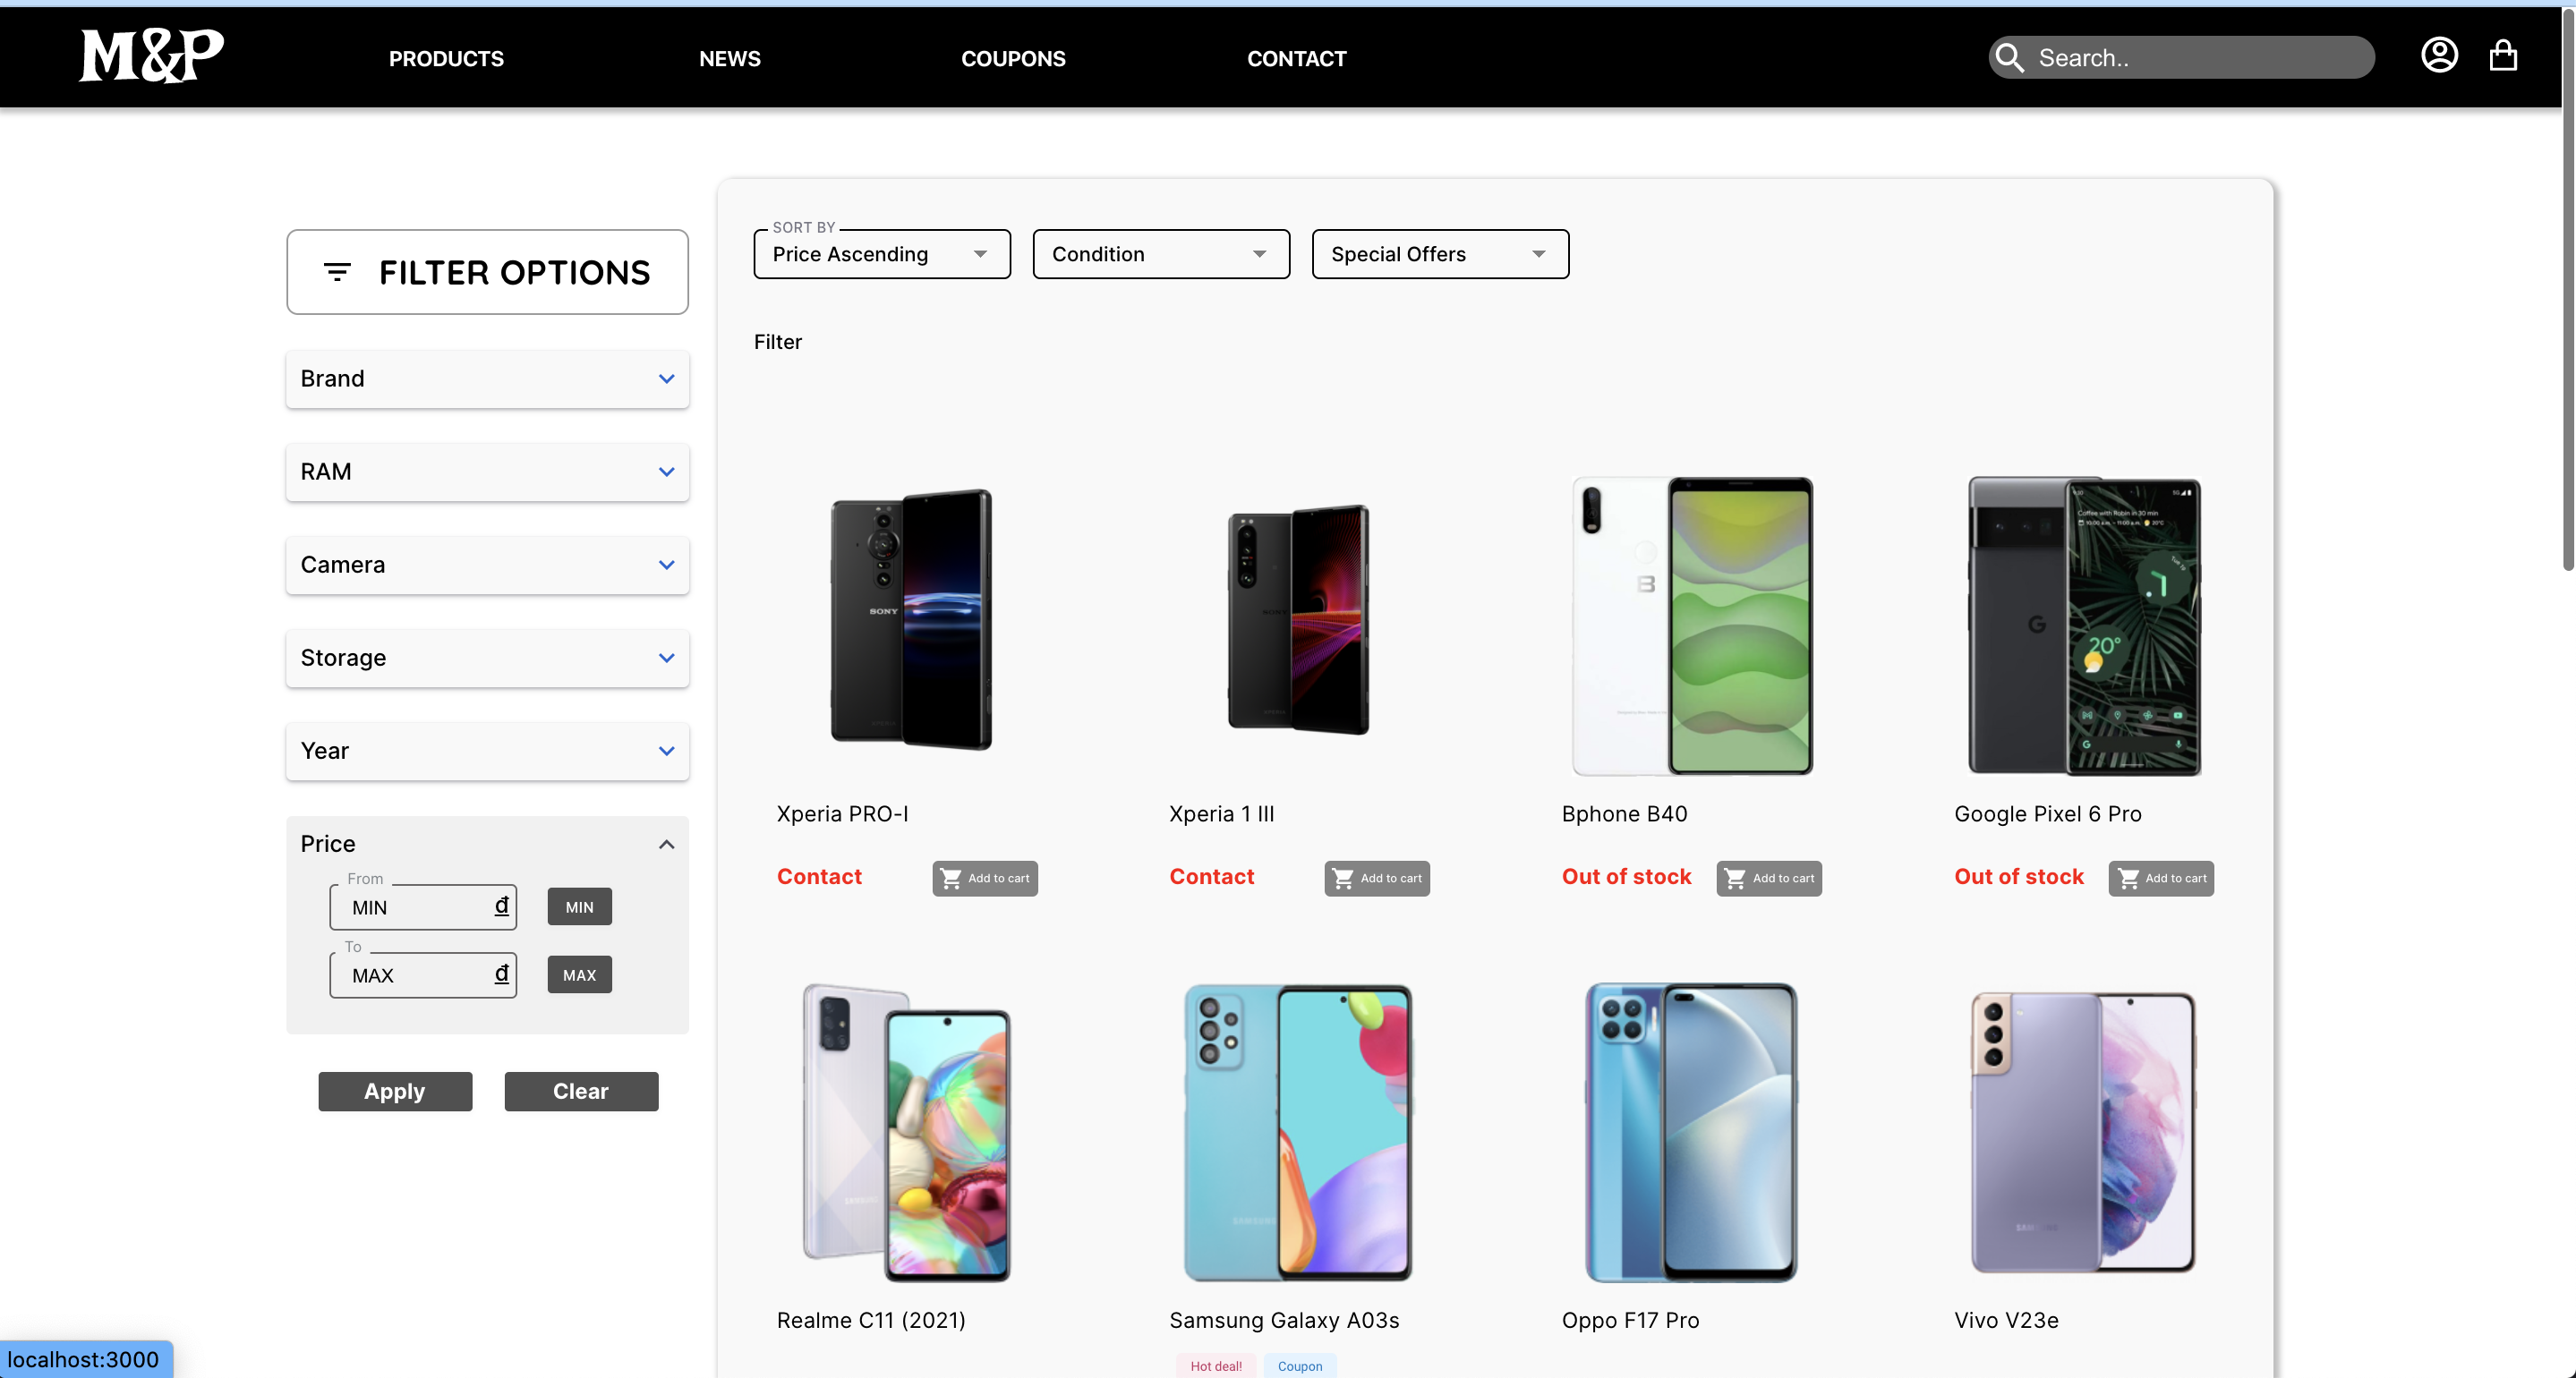
\includegraphics[width=0.9\textwidth]{assets/flow/product.png}
  \caption{Product List Page}
\end{figure}

The filter list is initially collapsed, and will be expanded if clicked.
The price range can be indicated as well.
After clicking the {\tt Apply} button, the page will be refreshed and the filtered will be applied.
If the {\tt Clear} button is clicked, all of the filters will be cleared.
After filter is applied, the filter options are also displayed.

\begin{figure}[H]
  \centering
  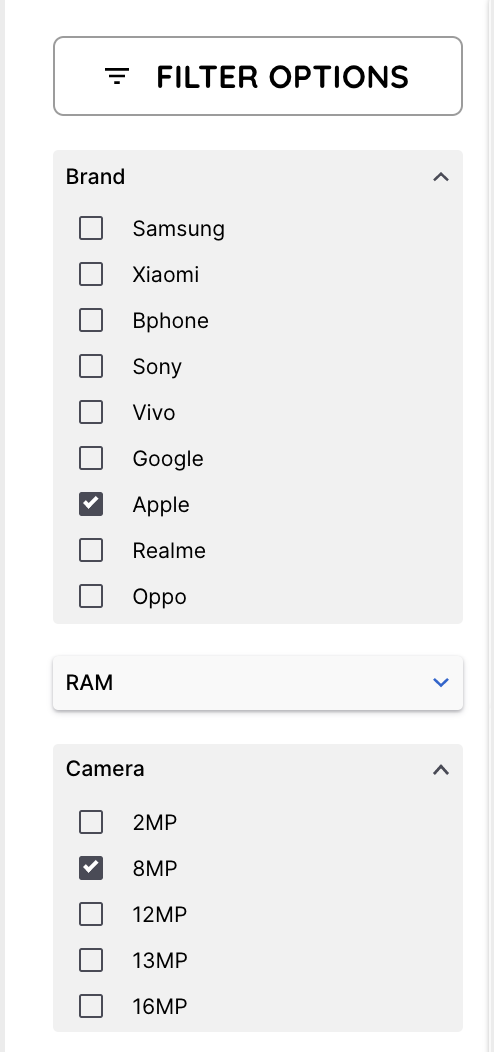
\includegraphics[width=0.2\textwidth]{assets/flow/filter1.png}
  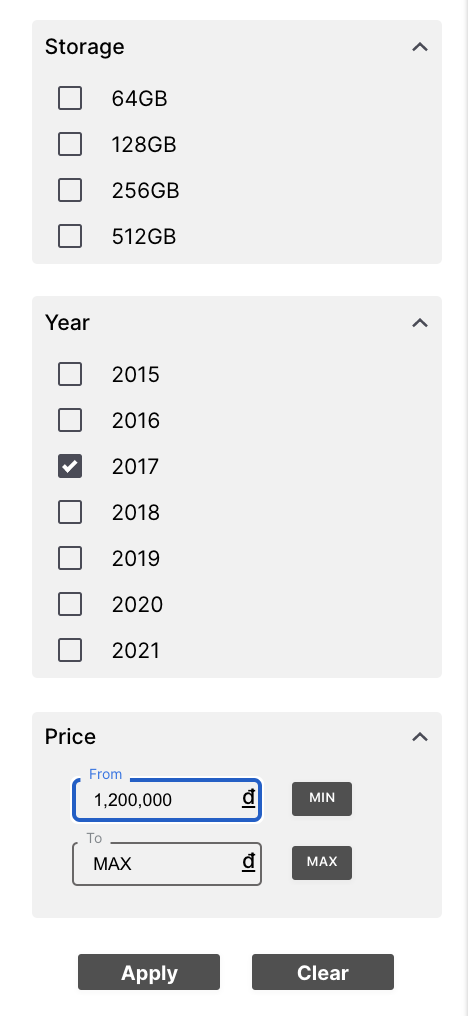
\includegraphics[width=0.2\textwidth]{assets/flow/price1.png}
  \caption{The filter column}
\end{figure}

\begin{figure}[H]
  \centering
  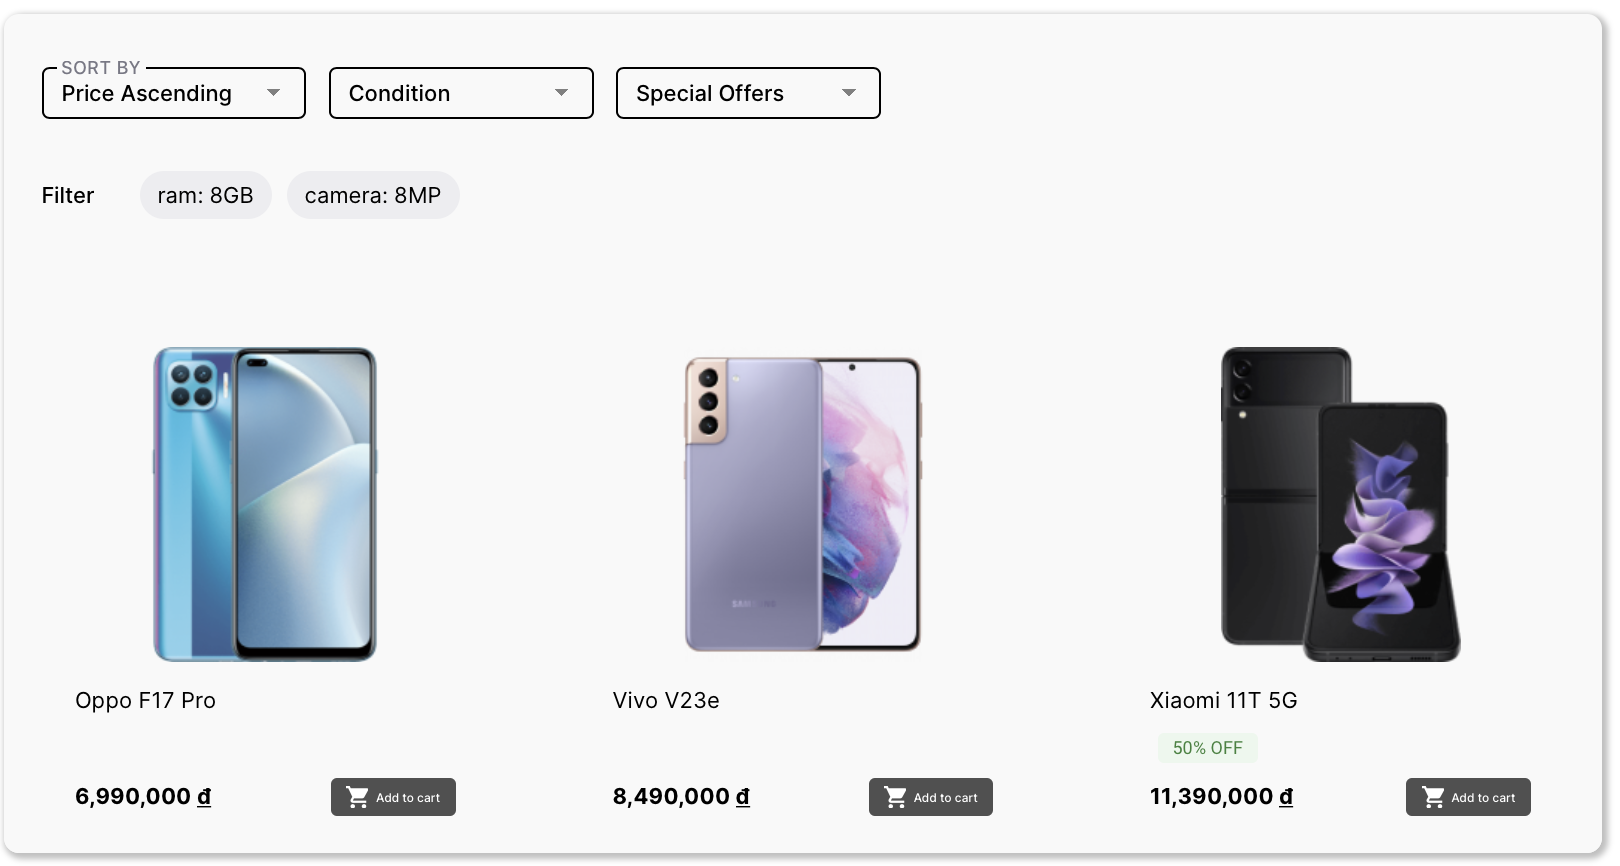
\includegraphics[width=0.9\textwidth]{assets/flow/filtered.png}
  \caption{Filter by RAM: 8GB and camera: 8MP}
\end{figure}

There is also a row to sort the products by price, filter the products by their condition and special offers.
A product will pop up if we hover the mouse over it.
For each product, we can view its name, price, and image.
If the product is {\tt Out of stock} or its price is not available, the price will be replaced with its condition.
If the products come with one or more special offers, its perks will also be included.
Users can also add items to their cart in this page.

\begin{figure}[H]
  \centering
  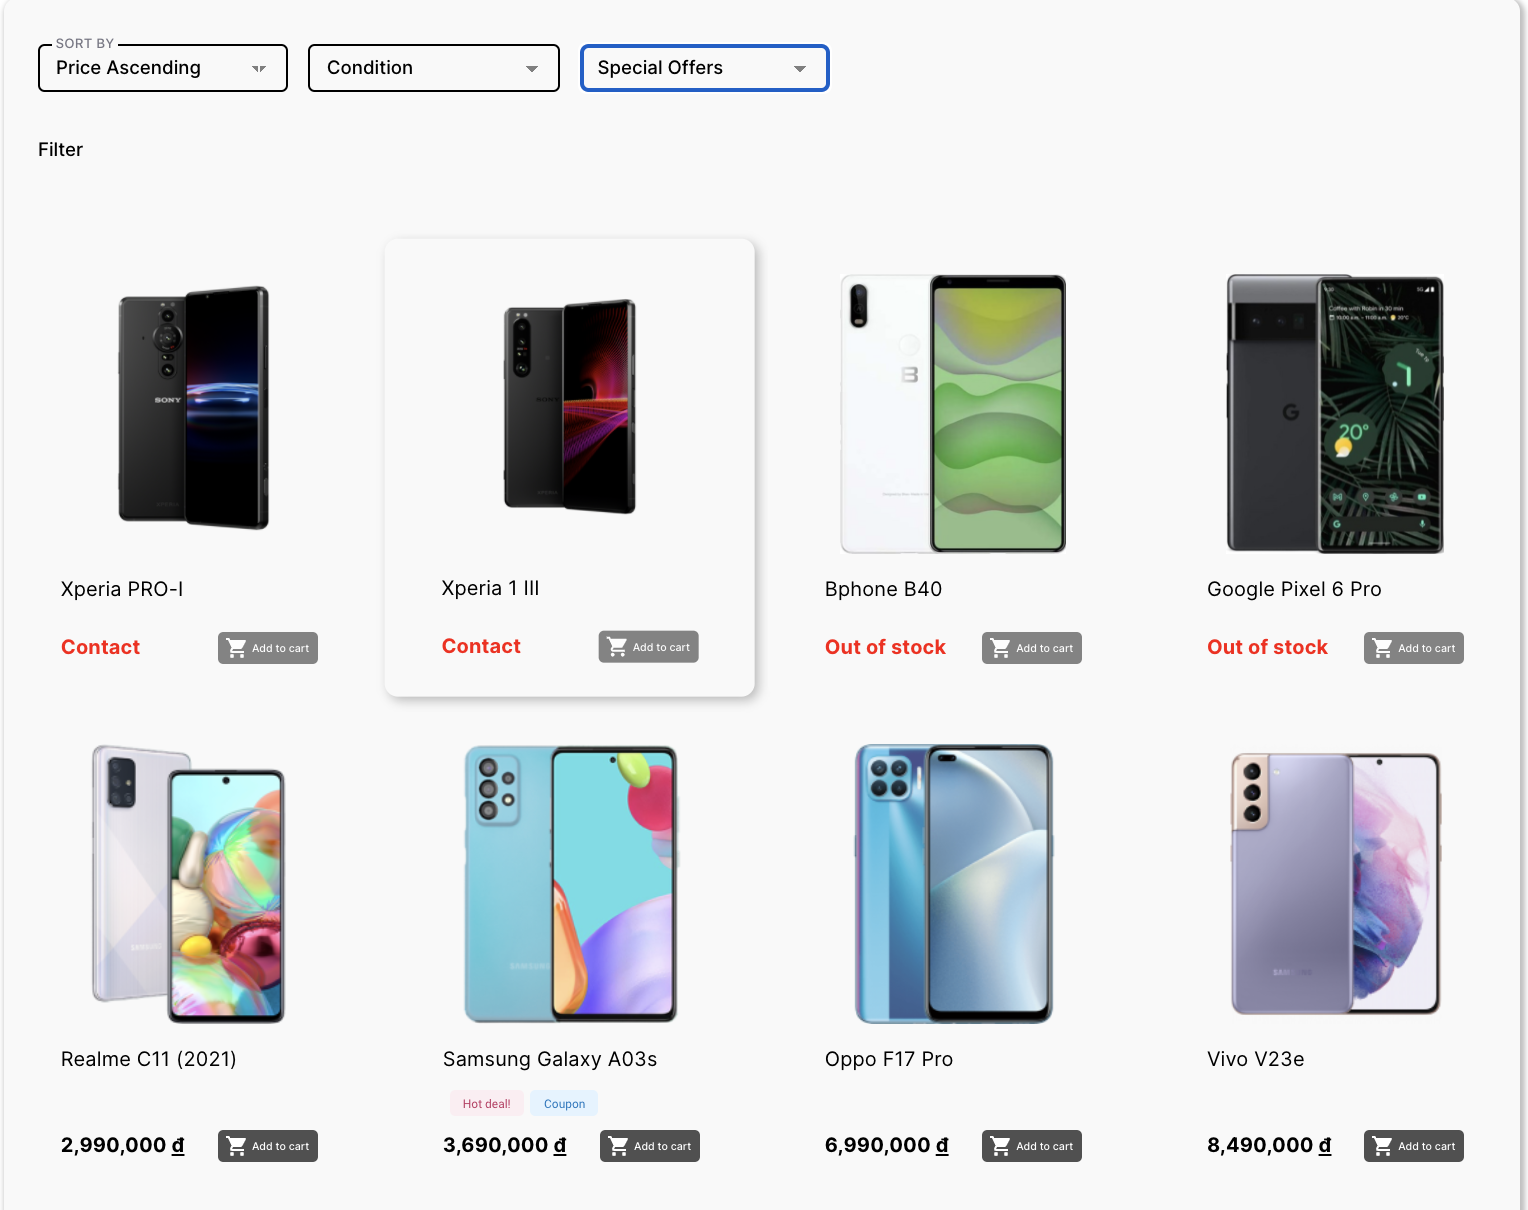
\includegraphics[width=0.8\textwidth]{assets/flow/prod.png}
  \caption{Close-up of the Product Page}
\end{figure}

\newpage
\subsection{Product Detail Page}

By clicking on an image of a product, users will be navigated to this page, which contains more information.
The {\tt Brand} card shows a general description of the phone's brand.
The table provides detail specifications.
Since inputting the correct detail is quite problematic, sometimes we only placed some random passages.\\

Each product is associated with a different list of storage and color options.
Users can choose from the options, and those chosen will be emphasized.
If the user clicks the {\tt Add to cart} button, it will simply add the item to their cart, and they can check immediately by clicking on the cart icon on the navigation bar.
By clicking the {\tt Buy now} button, the item is not only added to cart, the page is also directed to the {\tt Check Out Page}.

On the bottom of the page, there is also a list of related products.
These products are not fixed, they are randomly generated every time.

\begin{figure}[H]
  \centering
  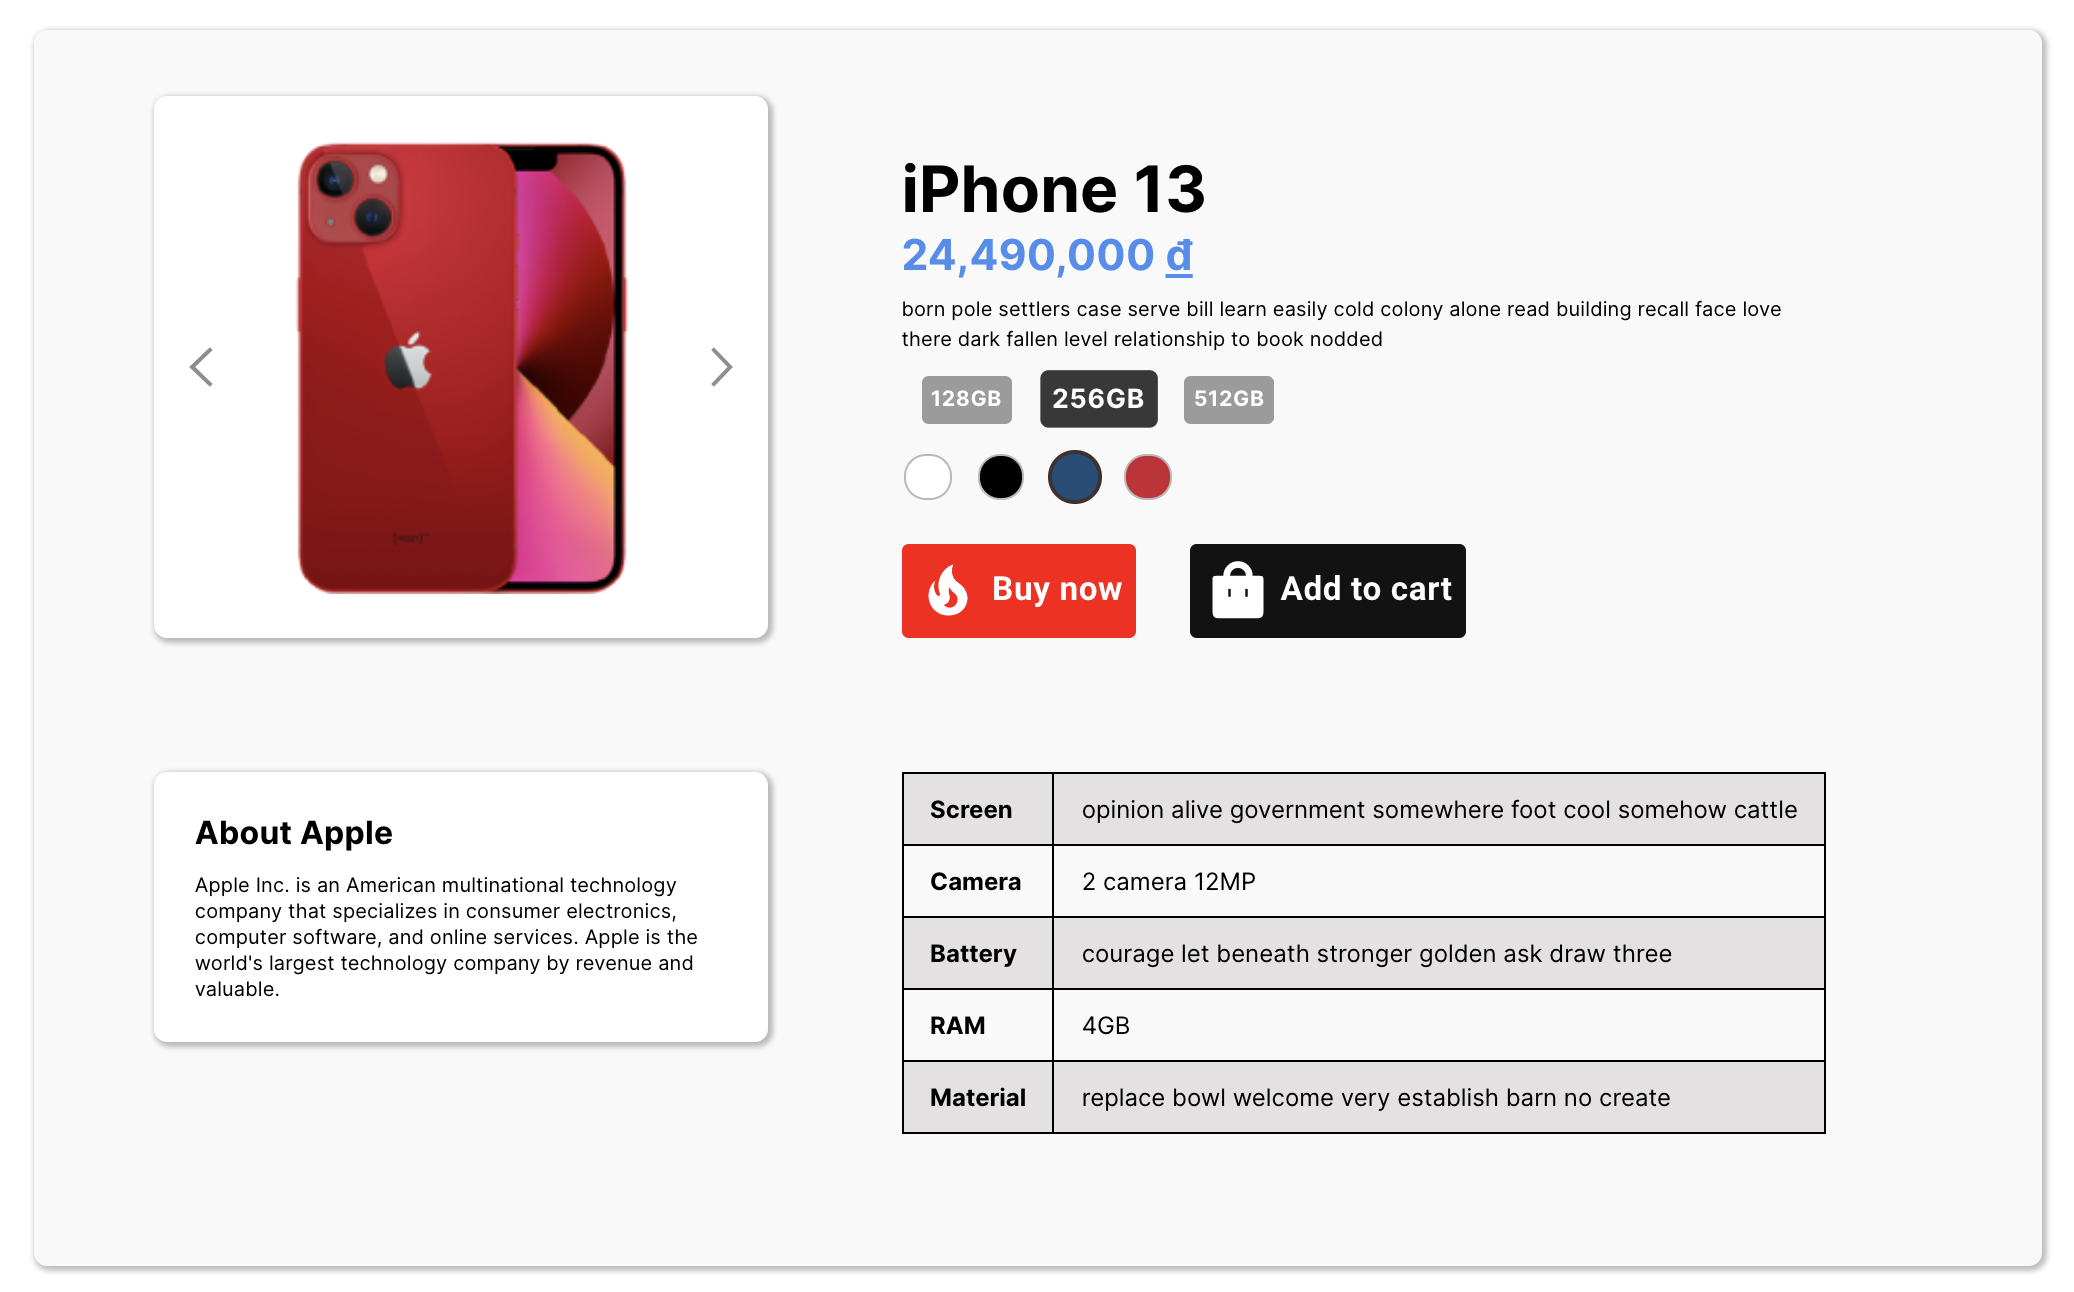
\includegraphics[width=0.9\textwidth]{assets/flow/detail.png}
  \caption{Product Detail Page}
\end{figure}

\begin{figure}[H]
  \centering
  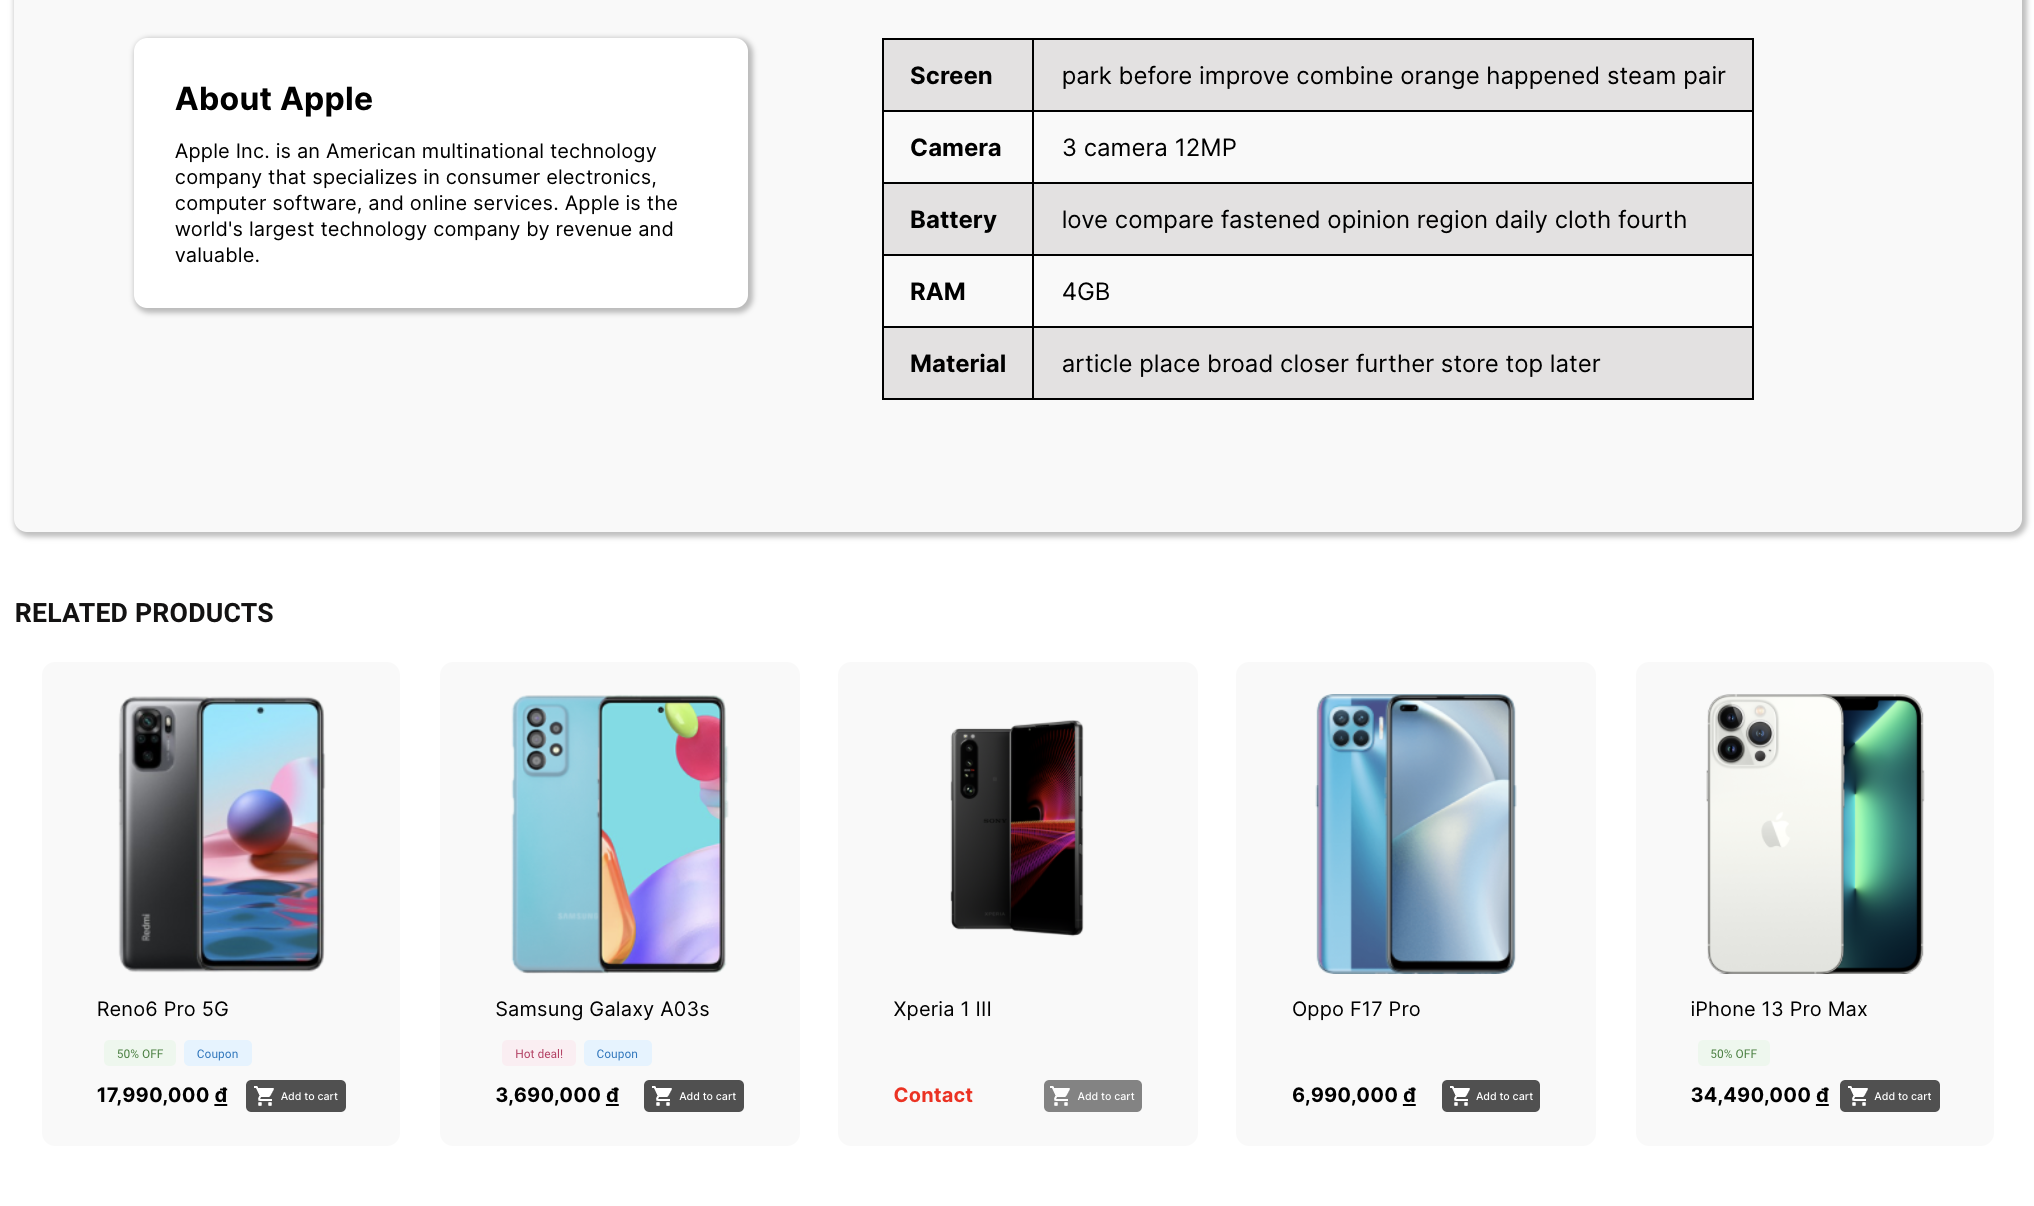
\includegraphics[width=0.9\textwidth]{assets/flow/related.png}
  \caption{Related Products}
\end{figure}

\newpage
\subsection{Check Out Page}
Finally, users can check out at this page after they signed in and have one or more products in the cart.
Users can modified the quantities of the existing products and can remove them at this stage.
The total price will be calculated for them.

\begin{figure}[H]
  \centering
  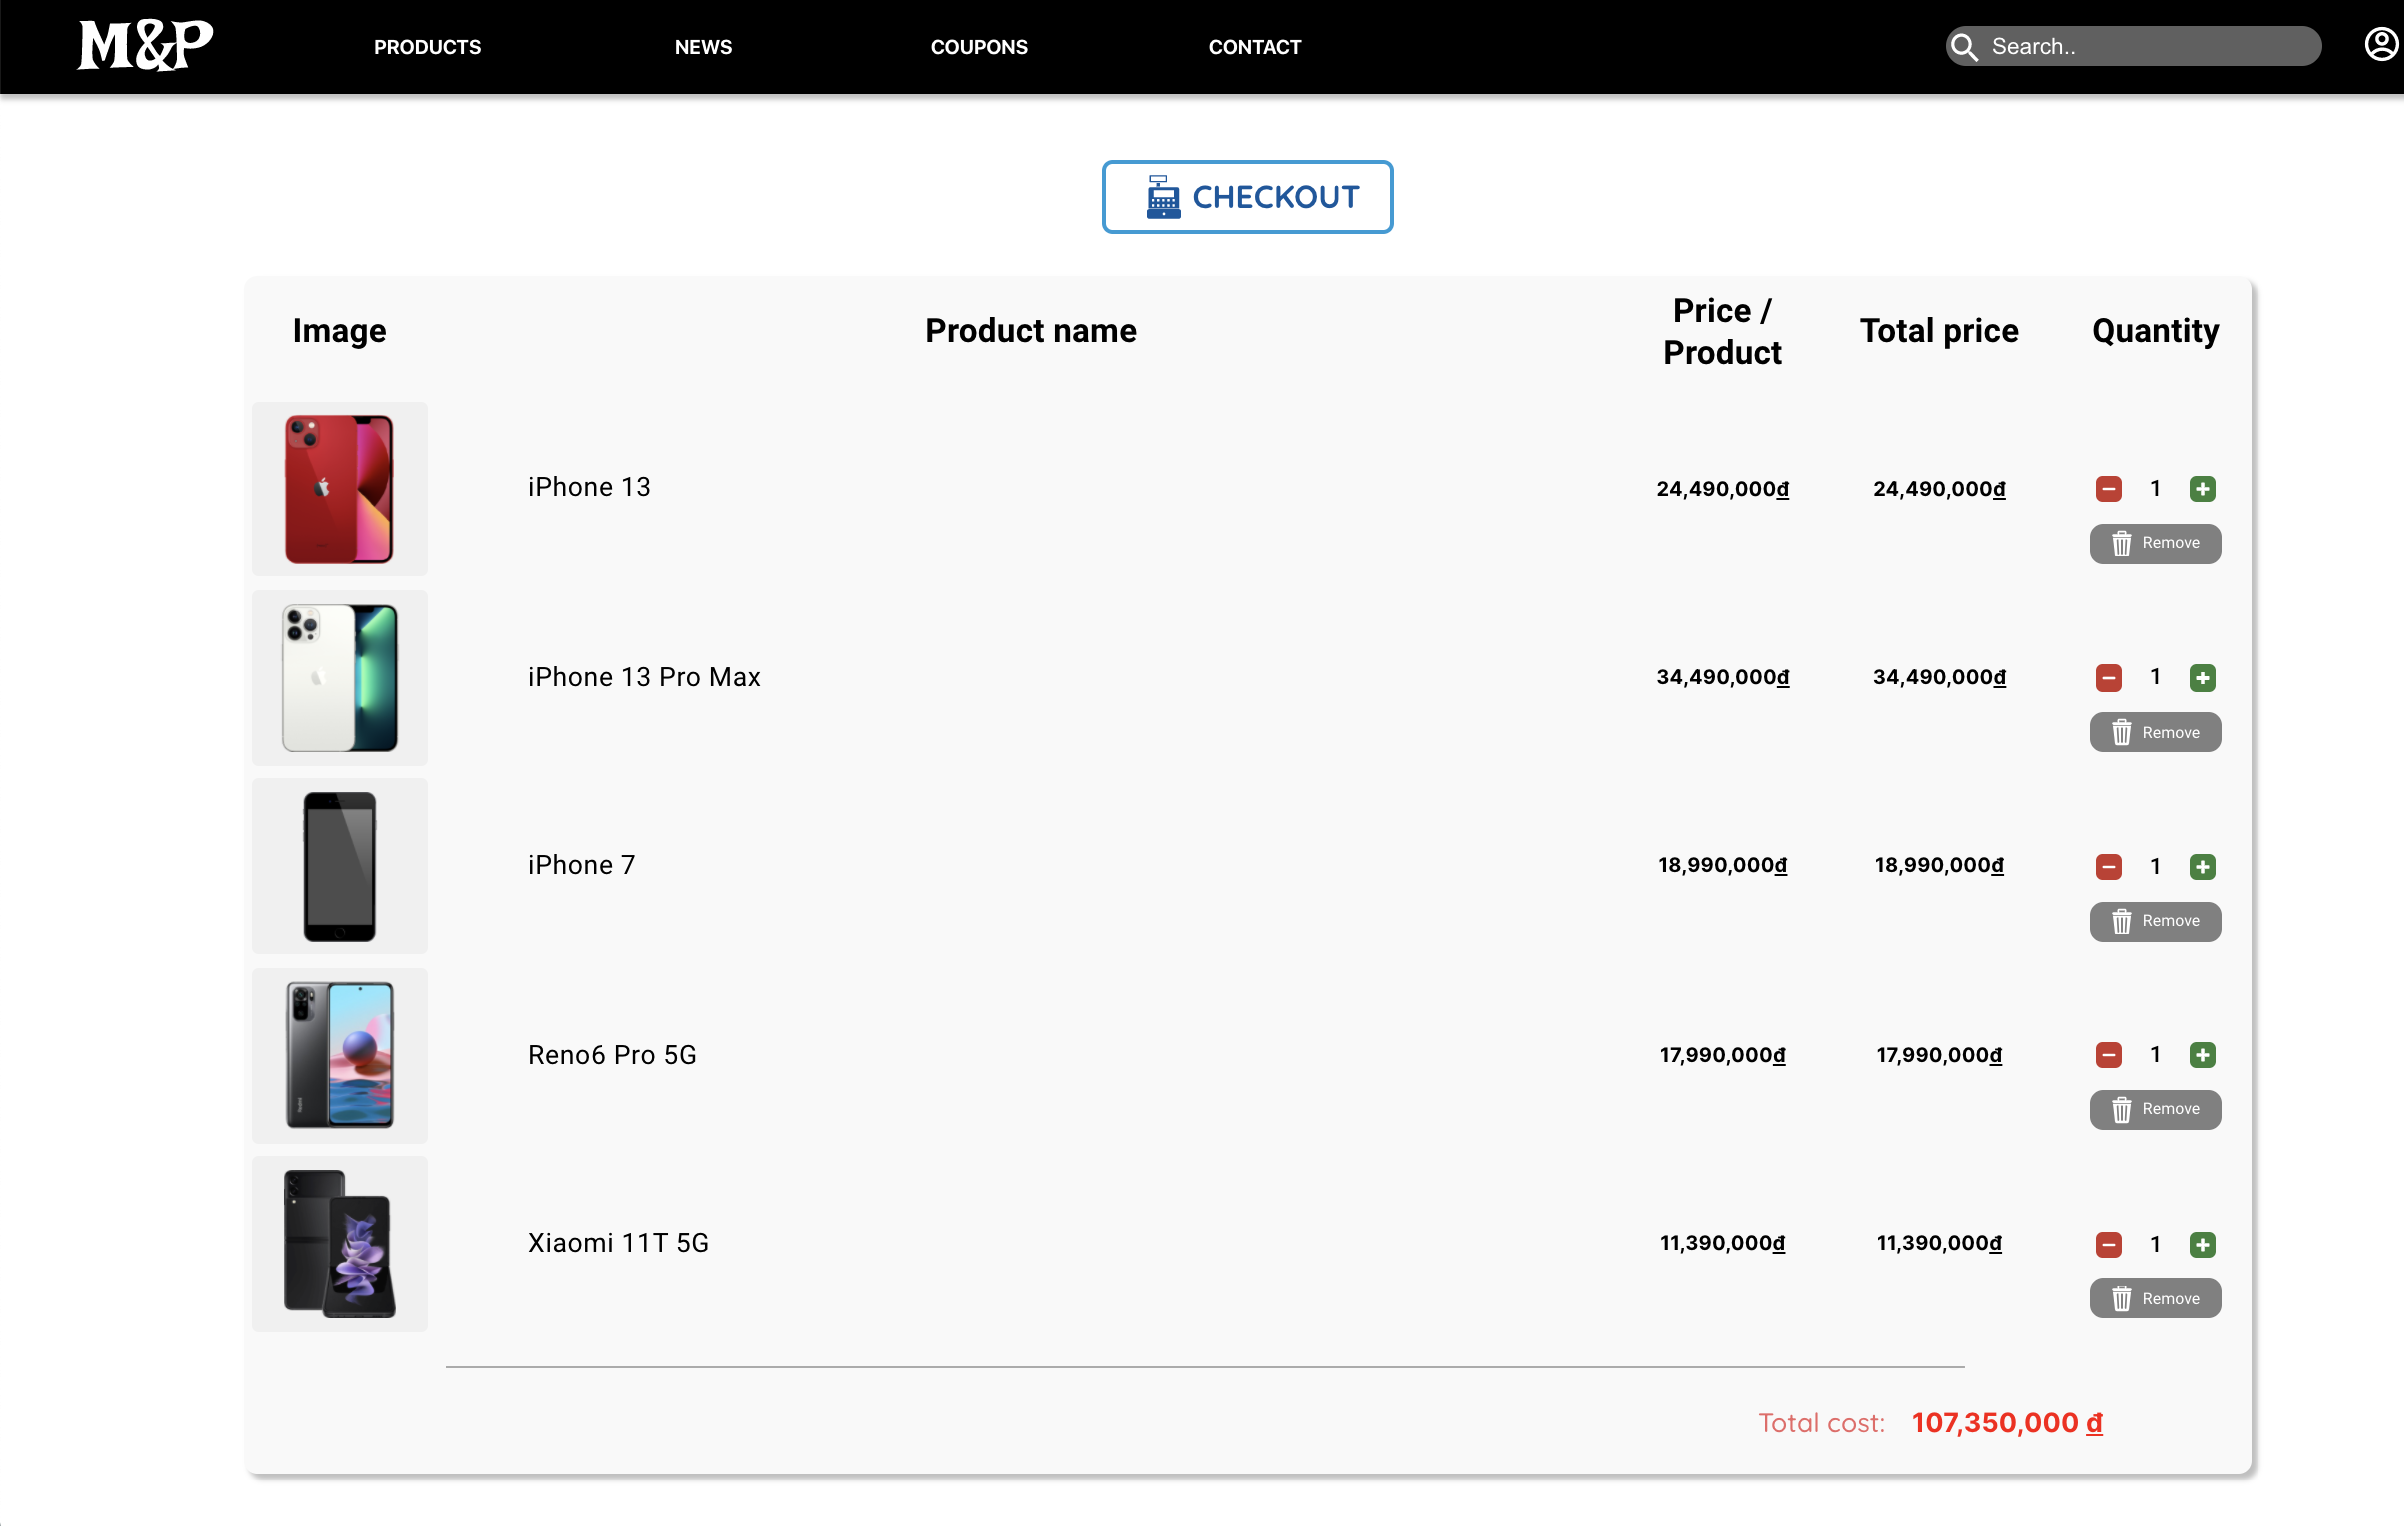
\includegraphics[width=0.9\textwidth]{assets/flow/cart.png}
  \caption{Check Out Page}
\end{figure}

Below that, there is a simple form which is halfway filled in by the information provided when users signed up an account.
At this stage, he/she needs to fill in the correct address, choose a payment option, then click {\tt Proceed}.
An alert will show up indicating that the simulation is successful, and an order placement activity ends here.

\begin{figure}[H]
  \centering
  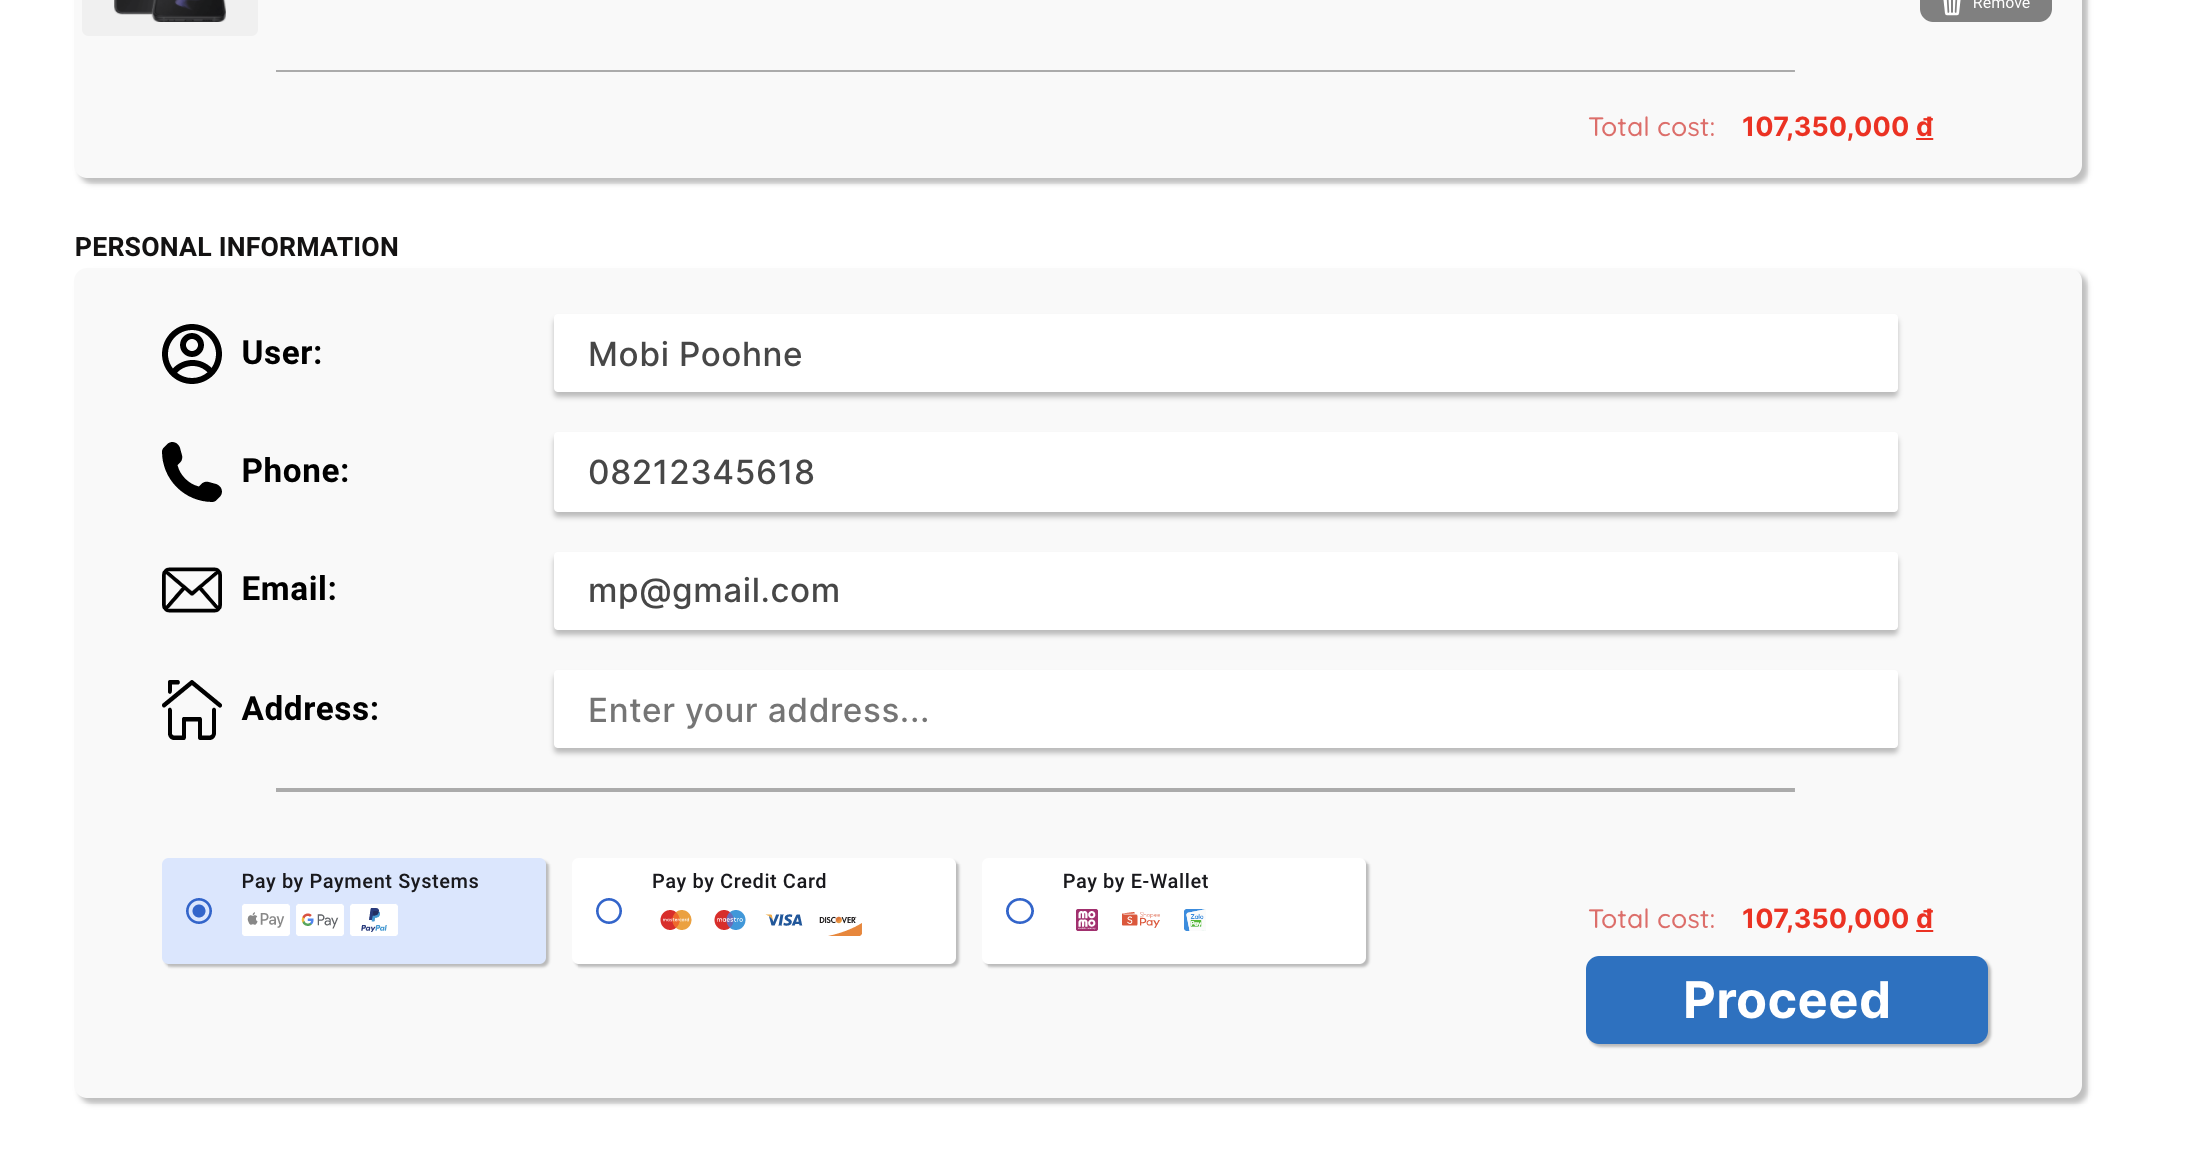
\includegraphics[width=0.9\textwidth]{assets/flow/form.png}
  \caption{Check Out Form}
\end{figure}

\end{document}
